
%% bare_jrnl.tex
%% V1.4b
%% 2015/08/26
%% by Michael Shell
%% see http://www.michaelshell.org/
%% for current contact information.
%%
%% This is a skeleton file demonstrating the use of IEEEtran.cls
%% (requires IEEEtran.cls version 1.8b or later) with an IEEE
%% journal paper.
%%
%% Support sites:
%% http://www.michaelshell.org/tex/ieeetran/
%% http://www.ctan.org/pkg/ieeetran
%% and
%% http://www.ieee.org/

%%*************************************************************************
%% Legal Notice:
%% This code is offered as-is without any warranty either expressed or
%% implied; without even the implied warranty of MERCHANTABILITY or
%% FITNESS FOR A PARTICULAR PURPOSE! 
%% User assumes all risk.
%% In no event shall the IEEE or any contributor to this code be liable for
%% any damages or losses, including, but not limited to, incidental,
%% consequential, or any other damages, resulting from the use or misuse
%% of any information contained here.
%%
%% All comments are the opinions of their respective authors and are not
%% necessarily endorsed by the IEEE.
%%
%% This work is distributed under the LaTeX Project Public License (LPPL)
%% ( http://www.latex-project.org/ ) version 1.3, and may be freely used,
%% distributed and modified. A copy of the LPPL, version 1.3, is included
%% in the base LaTeX documentation of all distributions of LaTeX released
%% 2003/12/01 or later.
%% Retain all contribution notices and credits.
%% ** Modified files should be clearly indicated as such, including  **
%% ** renaming them and changing author support contact information. **
%%*************************************************************************


% *** Authors should verify (and, if needed, correct) their LaTeX system  ***
% *** with the testflow diagnostic prior to trusting their LaTeX platform ***
% *** with production work. The IEEE's font choices and paper sizes can   ***
% *** trigger bugs that do not appear when using other class files.       ***                          ***
% The testflow support page is at:
% http://www.michaelshell.org/tex/testflow/



\documentclass[journal]{IEEEtran}
%
% If IEEEtran.cls has not been installed into the LaTeX system files,
% manually specify the path to it like:
% \documentclass[journal]{../sty/IEEEtran}
\newcounter{MYtempeqncnt}




% Some very useful LaTeX packages include:
% (uncomment the ones you want to load)


% *** MISC UTILITY PACKAGES ***
%
%\usepackage{ifpdf}
% Heiko Oberdiek's ifpdf.sty is very useful if you need conditional
% compilation based on whether the output is pdf or dvi.
% usage:
% \ifpdf
%   % pdf code
% \else
%   % dvi code
% \fi
% The latest version of ifpdf.sty can be obtained from:
% http://www.ctan.org/pkg/ifpdf
% Also, note that IEEEtran.cls V1.7 and later provides a builtin
% \ifCLASSINFOpdf conditional that works the same way.
% When switching from latex to pdflatex and vice-versa, the compiler may
% have to be run twice to clear warning/error messages.






% *** CITATION PACKAGES ***
%
\usepackage{cite}
% cite.sty was written by Donald Arseneau
% V1.6 and later of IEEEtran pre-defines the format of the cite.sty package
% \cite{} output to follow that of the IEEE. Loading the cite package will
% result in citation numbers being automatically sorted and properly
% "compressed/ranged". e.g., [1], [9], [2], [7], [5], [6] without using
% cite.sty will become [1], [2], [5]--[7], [9] using cite.sty. cite.sty's
% \cite will automatically add leading space, if needed. Use cite.sty's
% noadjust option (cite.sty V3.8 and later) if you want to turn this off
% such as if a citation ever needs to be enclosed in parenthesis.
% cite.sty is already installed on most LaTeX systems. Be sure and use
% version 5.0 (2009-03-20) and later if using hyperref.sty.
% The latest version can be obtained at:
% http://www.ctan.org/pkg/cite
% The documentation is contained in the cite.sty file itself.






% *** GRAPHICS RELATED PACKAGES ***
%
\usepackage{subcaption} % for subfigures
\ifCLASSINFOpdf
   \usepackage[pdftex]{graphicx}
  % declare the path(s) where your graphic files are
  % \graphicspath{{../pdf/}{../jpeg/}}
  % and their extensions so you won't have to specify these with
  % every instance of \includegraphics
  % \DeclareGraphicsExtensions{.pdf,.jpeg,.png}
\else
  % or other class option (dvipsone, dvipdf, if not using dvips). graphicx
  % will default to the driver specified in the system graphics.cfg if no
  % driver is specified.
  % \usepackage[dvips]{graphicx}
  % declare the path(s) where your graphic files are
  % \graphicspath{{../eps/}}
  % and their extensions so you won't have to specify these with
  % every instance of \includegraphics
  % \DeclareGraphicsExtensions{.eps}
\fi
% graphicx was written by David Carlisle and Sebastian Rahtz. It is
% required if you want graphics, photos, etc. graphicx.sty is already
% installed on most LaTeX systems. The latest version and documentation
% can be obtained at: 
% http://www.ctan.org/pkg/graphicx
% Another good source of documentation is "Using Imported Graphics in
% LaTeX2e" by Keith Reckdahl which can be found at:
% http://www.ctan.org/pkg/epslatex
%
% latex, and pdflatex in dvi mode, support graphics in encapsulated
% postscript (.eps) format. pdflatex in pdf mode supports graphics
% in .pdf, .jpeg, .png and .mps (metapost) formats. Users should ensure
% that all non-photo figures use a vector format (.eps, .pdf, .mps) and
% not a bitmapped formats (.jpeg, .png). The IEEE frowns on bitmapped formats
% which can result in "jaggedy"/blurry rendering of lines and letters as
% well as large increases in file sizes.
%
% You can find documentation about the pdfTeX application at:
% http://www.tug.org/applications/pdftex





% *** MATH PACKAGES ***
%
\usepackage{amsmath}
% A popular package from the American Mathematical Society that provides
% many useful and powerful commands for dealing with mathematics.
%
% Note that the amsmath package sets \interdisplaylinepenalty to 10000
% thus preventing page breaks from occurring within multiline equations. Use:
%\interdisplaylinepenalty=2500
% after loading amsmath to restore such page breaks as IEEEtran.cls normally
% does. amsmath.sty is already installed on most LaTeX systems. The latest
% version and documentation can be obtained at:
% http://www.ctan.org/pkg/amsmath





% *** SPECIALIZED LIST PACKAGES ***
%
%\usepackage{algorithmic}
% algorithmic.sty was written by Peter Williams and Rogerio Brito.
% This package provides an algorithmic environment fo describing algorithms.
% You can use the algorithmic environment in-text or within a figure
% environment to provide for a floating algorithm. Do NOT use the algorithm
% floating environment provided by algorithm.sty (by the same authors) or
% algorithm2e.sty (by Christophe Fiorio) as the IEEE does not use dedicated
% algorithm float types and packages that provide these will not provide
% correct IEEE style captions. The latest version and documentation of
% algorithmic.sty can be obtained at:
% http://www.ctan.org/pkg/algorithms
% Also of interest may be the (relatively newer and more customizable)
% algorithmicx.sty package by Szasz Janos:
% http://www.ctan.org/pkg/algorithmicx




% *** ALIGNMENT PACKAGES ***
%
\usepackage{array}
% Frank Mittelbach's and David Carlisle's array.sty patches and improves
% the standard LaTeX2e array and tabular environments to provide better
% appearance and additional user controls. As the default LaTeX2e table
% generation code is lacking to the point of almost being broken with
% respect to the quality of the end results, all users are strongly
% advised to use an enhanced (at the very least that provided by array.sty)
% set of table tools. array.sty is already installed on most systems. The
% latest version and documentation can be obtained at:
% http://www.ctan.org/pkg/array


% IEEEtran contains the IEEEeqnarray family of commands that can be used to
% generate multiline equations as well as matrices, tables, etc., of high
% quality.




% *** SUBFIGURE PACKAGES ***
%\ifCLASSOPTIONcompsoc
%  \usepackage[caption=false,font=normalsize,labelfont=sf,textfont=sf]{subfig}
%\else
%  \usepackage[caption=false,font=footnotesize]{subfig}
%\fi
% subfig.sty, written by Steven Douglas Cochran, is the modern replacement
% for subfigure.sty, the latter of which is no longer maintained and is
% incompatible with some LaTeX packages including fixltx2e. However,
% subfig.sty requires and automatically loads Axel Sommerfeldt's caption.sty
% which will override IEEEtran.cls' handling of captions and this will result
% in non-IEEE style figure/table captions. To prevent this problem, be sure
% and invoke subfig.sty's "caption=false" package option (available since
% subfig.sty version 1.3, 2005/06/28) as this is will preserve IEEEtran.cls
% handling of captions.
% Note that the Computer Society format requires a larger sans serif font
% than the serif footnote size font used in traditional IEEE formatting
% and thus the need to invoke different subfig.sty package options depending
% on whether compsoc mode has been enabled.
%
% The latest version and documentation of subfig.sty can be obtained at:
% http://www.ctan.org/pkg/subfig




% *** FLOAT PACKAGES ***
%
%\usepackage{fixltx2e}
% fixltx2e, the successor to the earlier fix2col.sty, was written by
% Frank Mittelbach and David Carlisle. This package corrects a few problems
% in the LaTeX2e kernel, the most notable of which is that in current
% LaTeX2e releases, the ordering of single and double column floats is not
% guaranteed to be preserved. Thus, an unpatched LaTeX2e can allow a
% single column figure to be placed prior to an earlier double column
% figure.
% Be aware that LaTeX2e kernels dated 2015 and later have fixltx2e.sty's
% corrections already built into the system in which case a warning will
% be issued if an attempt is made to load fixltx2e.sty as it is no longer
% needed.
% The latest version and documentation can be found at:
% http://www.ctan.org/pkg/fixltx2e


\usepackage{stfloats}
% stfloats.sty was written by Sigitas Tolusis. This package gives LaTeX2e
% the ability to do double column floats at the bottom of the page as well
% as the top. (e.g., "\begin{figure*}[!b]" is not normally possible in
% LaTeX2e). It also provides a command:
%\fnbelowfloat
% to enable the placement of footnotes below bottom floats (the standard
% LaTeX2e kernel puts them above bottom floats). This is an invasive package
% which rewrites many portions of the LaTeX2e float routines. It may not work
% with other packages that modify the LaTeX2e float routines. The latest
% version and documentation can be obtained at:
% http://www.ctan.org/pkg/stfloats
% Do not use the stfloats baselinefloat ability as the IEEE does not allow
% \baselineskip to stretch. Authors submitting work to the IEEE should note
% that the IEEE rarely uses double column equations and that authors should try
% to avoid such use. Do not be tempted to use the cuted.sty or midfloat.sty
% packages (also by Sigitas Tolusis) as the IEEE does not format its papers in
% such ways.
% Do not attempt to use stfloats with fixltx2e as they are incompatible.
% Instead, use Morten Hogholm'a dblfloatfix which combines the features
% of both fixltx2e and stfloats:
%
% \usepackage{dblfloatfix}
% The latest version can be found at:
% http://www.ctan.org/pkg/dblfloatfix




%\ifCLASSOPTIONcaptionsoff
%  \usepackage[nomarkers]{endfloat}
% \let\MYoriglatexcaption\caption
% \renewcommand{\caption}[2][\relax]{\MYoriglatexcaption[#2]{#2}}
%\fi
% endfloat.sty was written by James Darrell McCauley, Jeff Goldberg and 
% Axel Sommerfeldt. This package may be useful when used in conjunction with 
% IEEEtran.cls'  captionsoff option. Some IEEE journals/societies require that
% submissions have lists of figures/tables at the end of the paper and that
% figures/tables without any captions are placed on a page by themselves at
% the end of the document. If needed, the draftcls IEEEtran class option or
% \CLASSINPUTbaselinestretch interface can be used to increase the line
% spacing as well. Be sure and use the nomarkers option of endfloat to
% prevent endfloat from "marking" where the figures would have been placed
% in the text. The two hack lines of code above are a slight modification of
% that suggested by in the endfloat docs (section 8.4.1) to ensure that
% the full captions always appear in the list of figures/tables - even if
% the user used the short optional argument of \caption[]{}.
% IEEE papers do not typically make use of \caption[]'s optional argument,
% so this should not be an issue. A similar trick can be used to disable
% captions of packages such as subfig.sty that lack options to turn off
% the subcaptions:
% For subfig.sty:
% \let\MYorigsubfloat\subfloat
% \renewcommand{\subfloat}[2][\relax]{\MYorigsubfloat[]{#2}}
% However, the above trick will not work if both optional arguments of
% the \subfloat command are used. Furthermore, there needs to be a
% description of each subfigure *somewhere* and endfloat does not add
% subfigure captions to its list of figures. Thus, the best approach is to
% avoid the use of subfigure captions (many IEEE journals avoid them anyway)
% and instead reference/explain all the subfigures within the main caption.
% The latest version of endfloat.sty and its documentation can obtained at:
% http://www.ctan.org/pkg/endfloat
%
% The IEEEtran \ifCLASSOPTIONcaptionsoff conditional can also be used
% later in the document, say, to conditionally put the References on a 
% page by themselves.




% *** PDF, URL AND HYPERLINK PACKAGES ***
%
\usepackage{url}
% url.sty was written by Donald Arseneau. It provides better support for
% handling and breaking URLs. url.sty is already installed on most LaTeX
% systems. The latest version and documentation can be obtained at:
% http://www.ctan.org/pkg/url
% Basically, \url{my_url_here}.




% *** Do not adjust lengths that control margins, column widths, etc. ***
% *** Do not use packages that alter fonts (such as pslatex).         ***
% There should be no need to do such things with IEEEtran.cls V1.6 and later.
% (Unless specifically asked to do so by the journal or conference you plan
% to submit to, of course. )


% correct bad hyphenation here
\hyphenation{op-tical net-works semi-conduc-tor}


\begin{document}
%
% paper title
% Titles are generally capitalized except for words such as a, an, and, as,
% at, but, by, for, in, nor, of, on, or, the, to and up, which are usually
% not capitalized unless they are the first or last word of the title.
% Linebreaks \\ can be used within to get better formatting as desired.
% Do not put math or special symbols in the title.
\title{Performance Analysis of IEEE 802.11ax OFDMA-based Multi-Channel Random Access}
%
%
% author names and IEEE memberships
% note positions of commas and nonbreaking spaces ( ~ ) LaTeX will not break
% a structure at a ~ so this keeps an author's name from being broken across
% two lines.
% use \thanks{} to gain access to the first footnote area
% a separate \thanks must be used for each paragraph as LaTeX2e's \thanks
% was not built to handle multiple paragraphs
%

\author{Yang~Hang,
        Der-Jiunn~Deng,~\IEEEmembership{Member,~IEEE,} 
        and~Kwang-Cheng Chen,~\IEEEmembership{Fellow,~IEEE}% <-this % stops a space
\thanks{M. Shell was with the Department
of Electrical and Computer Engineering, Georgia Institute of Technology, Atlanta,
GA, 30332 USA e-mail: (see http://www.michaelshell.org/contact.html).}% <-this % stops a space
\thanks{J. Doe and J. Doe are with Anonymous University.}% <-this % stops a space
\thanks{Manuscript received April 19, 2005; revised August 26, 2015.}}

% note the % following the last \IEEEmembership and also \thanks - 
% these prevent an unwanted space from occurring between the last author name
% and the end of the author line. i.e., if you had this:
% 
% \author{....lastname \thanks{...} \thanks{...} }
%                     ^------------^------------^----Do not want these spaces!
%
% a space would be appended to the last name and could cause every name on that
% line to be shifted left slightly. This is one of those "LaTeX things". For
% instance, "\textbf{A} \textbf{B}" will typeset as "A B" not "AB". To get
% "AB" then you have to do: "\textbf{A}\textbf{B}"
% \thanks is no different in this regard, so shield the last } of each \thanks
% that ends a line with a % and do not let a space in before the next \thanks.
% Spaces after \IEEEmembership other than the last one are OK (and needed) as
% you are supposed to have spaces between the names. For what it is worth,
% this is a minor point as most people would not even notice if the said evil
% space somehow managed to creep in.



% The paper headers
\markboth{Journal of \LaTeX\ Class Files,~Vol.~14, No.~8, August~2015}%
{Shell \MakeLowercase{\textit{et al.}}: Bare Demo of IEEEtran.cls for IEEE Journals}
% The only time the second header will appear is for the odd numbered pages
% after the title page when using the twoside option.
% 
% *** Note that you probably will NOT want to include the author's ***
% *** name in the headers of peer review papers.                   ***
% You can use \ifCLASSOPTIONpeerreview for conditional compilation here if
% you desire.




% If you want to put a publisher's ID mark on the page you can do it like
% this:
%\IEEEpubid{0000--0000/00\$00.00~\copyright~2015 IEEE}
% Remember, if you use this you must call \IEEEpubidadjcol in the second
% column for its text to clear the IEEEpubid mark.



% use for special paper notices
%\IEEEspecialpapernotice{(Invited Paper)}




% make the title area
\maketitle

% As a general rule, do not put math, special symbols or citations
% in the abstract or keywords.
\begin{abstract}
%\boldmath
With the progressive increase of dense WiFi networks deployment, quality-of-experience (QoE) and power saving are becoming critical issues. 
IEEE 802.11ax, a task group aimed at high efficient WLAN (HEW), is to handle this dense scenario.
802.11ax makes revolutionary modifications to both MAC and PHY layer. 
One of the main features is OFDMA-based random access mechanism.
We extend the Markov chain model \cite{bianchi2000performance} to precisely describe the steady state behavior of the OFDMA-based random access.
Also, system efficiency and access delay of the random access mechanism are derived. 
Finally, we estimate the effects of system parameters, including number of resource units (RUs) for random access, initial and maximum contention window.
\end{abstract}
% IEEEtran.cls defaults to using nonbold math in the Abstract.
% This preserves the distinction between vectors and scalars. However,
% if the journal you are submitting to favors bold math in the abstract,
% then you can use LaTeX's standard command \boldmath at the very start
% of the abstract to achieve this. Many IEEE journals frown on math
% in the abstract anyway.

% Note that keywords are not normally used for peerreview papers.
\begin{IEEEkeywords}
MCRA, Multi-User PHY, OFDMA, 802.11ax
\end{IEEEkeywords}






% For peer review papers, you can put extra information on the cover
% page as needed:
% \ifCLASSOPTIONpeerreview
% \begin{center} \bfseries EDICS Category: 3-BBND \end{center}
% \fi
%
% For peerreview papers, this IEEEtran command inserts a page break and
% creates the second title. It will be ignored for other modes.
\IEEEpeerreviewmaketitle
% not use reference
%\cite{khorov2015survey}
\section{Introduction}		\label{Intro}

% what is dense scenario
During last decades, IEEE 802.11 achieved great success, enormous WiFi networks have been deployed because of its high throughput and relative simplicity of implementation.
According to Cisco Visual Network index \cite{cisco2016}, the mobile traffic will increase 53\% at CAGR within 2015-
2020, i.e., eight-fold, reaching 30.6 EB per month by 2020.
Therefore, scenarios of WiFi networks will become the \textit{dense scenarios}, which means plenty of stations (STA) or access points (AP) or both exist in a limited area. 
In this paper, we only focus on case of single AP with multiple STAs. 

% history of 802.11 i.e., legacy solutions not work, MAC is bottleneck
Actually, a series of standards, 802.11b, g, n, ac, have evolved to handle the increasing WLAN usage.
The method is mainly by means of raising data rate on physical layer (PHY)  from 2 Mbps to 7 Gbps \cite{perahia2013next}.
However, performance or user experience of WiFi networks dose not improve enough with the data rate, especially in dense scenario. 
That is because bottleneck of dense WiFi networks gradually relocate at MAC layer.
The MAC is always based on distributed coordination function (DCF), which is a random access protocol. 
Compared with that on PHY layer, legacy 802.11 made fewer changes on MAC layer. 
Collisions consume much efficiency in dense scenario.

% causes of bottleneck at MAC
MAC efficiency is wasted by two parts, overhead of control signaling and collisions.
Much effort has been conducted in legacy 802.11 to reduce the overhead of control signaling, such as RIFS, frame aggregation, etc \cite{perahia2013next}. 
In dense scenario, collisions will be the major component of spectrum waste.
That is why bottleneck relocate at MAC layer.
Collision is caused by two problems, instable distributed coordination function (DCF) problem and unfair queueing problem.

First, DCF is inherently instable as it is a random access protocol. 
Collisions will consume even more resource in dense scenario. 
Secondly, when we see the WiFi network with queueing model, WiFi network will be an unfair queue, which will worsen the effect of instability of DCF. 
%Each STA and AP are modeled as an individual queue, and the shared spectrum or the channel is seen as the server.
%Packets thus become the customers served by channel. 
%Because legacy 802.11 implement single-user (SU) channel. That means at one time, at most one packet could be served successfully; otherwise collision happens.
On the one hand, each STA and AP  (each queue) has the same chance to access the channel (server). 
On the other hand, because WiFi network operates in a star topology, AP as the center and STAs surrounding the AP logically, AP shares more than $1/2$ down-link (DL) traffic loading, while AP only has $1/(n+1)$ chance to access channel, where $n$ is the number of STAs.
The queue model of WiFi network is, therefore, an unfair queue between DL and up-link (UL) transmissions. 


% DCF to scheduled MAC, TF-based UL
Study group 802.11, target high efficiency WLAN (HEW) in dense scenario, thus modifies the MAC thoroughly, change DCF to central control. 
On PHY layer, OFDMA is issued to implement both DL and UL multi-user (MU) channel, which means a STA could communicate with multiple STAs at a time. 
On MAC layer, a brand new control frame called trigger frame (TF) is created to implement TF-based UL transmission. 
The AP thus could schedule both DL and UL transmissions, which means DCF will be replaced by a scheduled MAC protocol. 
And instability of DCF will be mitigated very well and unfair queueing problem will not exist any more as AP does not need to contend with STAs.
Moreover, a OFDMA-based multi-channel random access (MCRA) is proposed in 802.11ax as random access is highly efficient to transmit short frames, like bandwidth request. 
In this mechanism, AP initiates the MCRA by transmit a TF at first. 
STAs receiving the TF then contends with Aloha and binary exponential backoff mechanism. 
AP at last responds with ACK telling which STAs succeed in contending.
A random access procedure is thus composed of three-way handshake. 
Details will be illustrated in Section II.

% Related works of MCRA
As for the OFDMA-based MCRA, we are concerned about number of stations succeeding in accessing the channel and access delay.
Actually, MCRA has been supported by cellular networks to perform initial association to the network and to request transmission resources.
This is the first time for 802.11 to apply OFDMA shifting SU PHY to MU PHY.
However, cellular networks have adopted OFDMA for a while. 
Also OFDMA-based MCRA is solicited by cellular network for initial association and bandwidth request etc.
The OFDMA-based MCRA in cellular networks is conceptually the same with that of WiFi networks. 
In recent years, related works have proposed some models to derive the throughput \cite{zhou2008efficient}\cite{shen2003performance}\cite{choi2006multichannel}, the collision probability\cite{kim2012performance}\cite{seo2011design}, and the access delay \cite{zhou2008efficient}\cite{kim2012performance}\cite{seo2011design}\cite{behroozi1992delay}. 
\cite{zhou2008efficient} gives a closed-form expression of throughput for OFDMA system. 
\cite{shen2003performance} proposes a stabilized multi-channel slotted Aloha algorithm.
\cite{choi2006multichannel} designs a 1-persistent type retransmission, i.e., no exponential backoff, to achieve a fast access.
Some other works compare performance of two kinds of backoff mechanism, binary exponential backoff and uniform backoff  \cite{zhou2008efficient}\cite{seo2011design}\cite{kim2012performance}, which are implemented by IEEE 802.16 and 3GPP LTE respectively.  
\cite{wei2015modeling} specifies a model estimating transient behavior of OFDMA system.
In addition, \cite{GeneralizedOFDMACSMACA} generalizes CSMA/CA to OFDMA system for 802.11, which is much different from \cite{draft_ax}.


% Our contribution
In this paper, we estimate the steady state behavior of the OFDMA-based MCRA by extending Bianchi's Markov chain model.
Bianchi's model has never been shifted to model the OFDMA-based MCRA. 
Though the MCRA has big difference from DCF, including SU to MU channel, distributed scheme to central control scheme and listening before talk to Aloha, Bianchi's Markov chain model will have been validated that it precisely model the MCRA by some modifications.
Also, we evaluate system efficiency, access delay and effects of important system parameters. 

% organization
The paper is organized as follows.
More explanations of 802.11ax features are given in Section \ref{sec_ax_feature}, including MU UL/DL transmission procedure and OFDMA-based random access procedure.
Section \ref{sec_sys_model} contains the system model and performance analysis, system efficiency and access delay of the MCRA mechanism. 
Then Section \ref{sec_model_val} shows simulation results compared with analysis results, which validates the model.
Additional considerations on optimal performance are carried out in Section \ref{sec_max_min}. 
After that, Section \ref{sec_perf_eval} evaluates the performance and effects of important system parameters. 
Conclusion remark is given in Section \ref{sec_conclu}.


%% 
%%1. why 802.11ax, dense, DCF, contention, collision
%During last decades, IEEE 802.11 achieved great success. Enormous wifi networks have been deployed because of its high throughput and relative simplicity of implementation.
%The foundation of 802.11 MAC, distributed coordination function (DCF), is a random access protocol \cite{bianchi2000performance}.
%The DCF together with star topology of a 802.11 WLAN results in an unfair queueing. 
%Since in star topology,  access point (AP) needs to transmit all the down-link (DL) traffic, which is often more than $1/2$ traffic loading of the basic service set (BSS), while AP has only $1/n$ chance to access medium where $n$ is number of total stations including AP. It is, thus, an unfair queueing problem.
%What's worse, combining effect of the unstability of random access's nature and the unfair queueing problem, once under a dense scenario, the performance will degrade severely since contention and collision will occupy the channel.
%That lies the defect of legacy 802.11.
%We collectively call them dense deployment problem.
%The dense deployment problem not only degrades throughput but also waste much energy.
%
%%2. ax feature, MU, central control, but OFDMA-random access
%Previous amendments, 802.11n and 802.11ac called high throughput (HT) and very high throughput (VHT) respectively which are aimed at improving throughput, only mitigate the dense deployment problem. 
%The bottleneck at the MAC efficiency is not resolved.
%Thus, 802.11ax task group is issued targeted at high efficiency WLAN (HEW), improving quality of experience (QoE) and power save.
%Confronting the dense deployment problem, 802.11ax permits AP of central control, to schedule both down-link (DL) and up-link (UL) transmission so that contention is much reduced and unfair queueing problem could be resolved.
%IEEE 802.11ax also issues multi-user (MU) PHY which is supported with Orthogonal Frequency Multiple Access (OFDMA), and a special control frame called trigger frame (TF) to implement trigger-based MU UL\cite{draft_ax}. 
%Accordingly, multi-channel random access, the focus of this paper, is of course implemented in 802.11ax, named OFDMA-based random access, since random access is an efficient way for stations to transmit bandwidth request, buffer status report (BSR) etc. 
%Actually, the new MAC is based on DCF since it helps co-exist among BSS and other systems. The difference is that the DCF mainly works on AP which means AP needs to access channel following DCF procedure, while HE-STA (802.11ax STA) is mostly scheduled by AP and even the random access procedure is initialized by AP. 
%
%%3. related work, random acces history ? , clarify OFDMA-based random access is special
%% SU/MU; aloha/CSMA; BEB/UB; saturated/unsaturated
%Random access is a classical topic in data network.
%It originates from Aloha and slotted Aloha \cite{abramson1970aloha}, which are also named collision resolution, with single-user channel. 
%Inherently, collision resolution algorithms can achieve small delay with a large number of lightly loaded nodes \cite{bertsekas1992data}.
%Then CSMA works as typical collision resolution  \cite{kleinrock1975packet}\cite{chen1994medium}, which is accepted by IEEE 802.11 named CSMA/CA \cite{bianchi2000performance}. 
%CSMA/CA has been a popular approach to MAC on unlicensed band for a long time, since it is easily implemented and robust. 
%For random access, the stability is a major concern. 
%% MU PHY
%With the emergence of MU PHY techniques, like MU-MIMO or MU-OFDMA, multi-user (MU) channel random access is proposed.
%We concern about MU-OFDMA.
%With MU channel, randomness extends from time domain to time-frequency domain, 2-dimension.
%The MU random access is mainly adopted by cellular networks, IEEE 802.16 and 3GPP LTE.
%And cellular network only implements random access for initial up-link access. 
%In recent years, several analytical models have been proposed to derive the throughput \cite{zhou2008efficient}\cite{shen2003performance}\cite{choi2006multichannel}, the collision probability\cite{kim2012performance}\cite{seo2011design}, and the access delay \cite{zhou2008efficient}\cite{kim2012performance}\cite{seo2011design}\cite{behroozi1992delay}. 
%In \cite{kim2012performance}, the authors presented an analytical model to evaluate the access success probability and the access delay for UMTS system.
%\cite{choi2006multichannel} designs a 1-persistent type retransmission, i.e., no exponential backoff, to achieve a fast access.  
%In \cite{zhou2008efficient}, a closed-form expression of throughput for OFDMA system is firstly given.
%
%% backoff mechanism
%The backoff mechanism, which is about retransmission when failure occurs, is also important in random access.
%Many works compare performance of two backoff mechanism, binary exponential backoff and uniform backoff  \cite{zhou2008efficient}\cite{seo2011design}\cite{kim2012performance}, which are implemented by IEEE 802.16 and 3GPP LTE respectively.  \cite{wei2015modeling} specifies a model estimating transient behavior of OFDMA system.
%
%%many metrics: throughput, mean and variance of access delay, stability
%All above works about OFDMA random access is an Aloha-type access in cellular network.
%In addition, \cite{GeneralizedOFDMACSMACA} is one of a few works for 802.11. It generalizes CSMA/CA to OFDMA system for 802.11.
%
%%4. our work
%% the first to analyze the 802.11ax random access
%Though OFDMA and multi-channel random access have been employed by IEEE 802.16 and 3GPP LTE for a long time.
%It is the first time for 802.11ax to issue OFDMA and OFDMA-based random access, which is a huge evolution for 802.11.
%And as far as we know, this is the first paper analyzing IEEE 802.11ax OFDMA-based random access. 
%It employs binary exponential backoff and MU PHY under Trigger-based MU UL, which is different from \cite{GeneralizedOFDMACSMACA}.
%Since \cite{bianchi2000performance} proposes an accurate Markov chain model for DCF, we could also reuse this model to generate another Markov chain for 802.11ax to precisely depict the OFDMA-based random access.
%We assume stations are under saturated condition which means they always have packets to transmit.
%The saturated analysis is based on the key assumption of independent collision probability $p$ whatever the packet is retransmitted or not.
%Simulation validates our model to be accurate.
%Then, we estimate the maximum system efficiency and minimum access delay. 
%Since OFDMA-based random access has dynamic and more complicated parameter sets than legacy 802.11, we evaluate effect of a variety of parameter sets and at last propose rules for AP to configure the parameter set. 
%
%The paper is organized as follows.
%More explanations of 802.11ax features are given in section \ref{sec_ax_feature}. 
%In section \ref{sec_RA_illu}, a detailed illustration of OFDMA-based random access procedure is presented.
%Section \ref{sec_sys_model} contains the system model and performance analysis, including system efficiency and access delay, of the random access mechanism. 
%Then section \ref{sec_model_val} shows simulation results compared with analysis results, which validates the model.
%In section \ref{sec_max_min}, additional considerations on optimal performance are carried out. 
%Section \ref{sec_perf_eval} gives performance evaluation under various parameter sets and at last propose rules for configuring the parameter set.
%Conclusion remark is given in section \ref{sec_conclu}.


\section{802.11ax Features}			\label{sec_ax_feature}
% 1. OFDMA MU, 2. TF-based UL 3. DCF to centralized coordination function
In this section, necessary features of 802.11ax will be illustrated to understand the OFDMA-based MCRA mechanism.
As stated above, collisions in dense scenario degrade performance of WiFi networks as the bottleneck locates at MAC.
Study group 802.11ax thus proposes TF-based UL procedure, which means AP schedules both DL/UL transmissions.
In respect of DL/UL, 802.11ax shifted the distributed coordination legacy 802.11 to centralized coordination.
on the other hand, OFDMA is issued in IEEE 802.11ax to realize MU PHY.
Additionally, OFDMA-based multi-channel random access (MCRA) is proposed.
For more features of 802.11ax, \cite{dengquality} is a good reference.

\subsection{PHY}
With MU PHY, the original SU 20 MHz channel could be specified more fine-grained and also aggregated to a wider channel.
The resource unit (RU), which can be accessed by one STA, is specified as Figure \ref{fig_RU_spec}. The smallest RU is 26-tone, with which a 20 MHz could be separated into 9 subchannels.
Also, coarse-grained RU is accepted.
And as specified in Figure \ref{fig_RU_spec}, multiple 20 MHz channels can be aggregated, which is called \textit{Channel Bonding}. 
This will help improve system performance, since one BSS is not restricted to a single 20 MHz channel.  
It is worth mentioning that every transmission of MU should end at the same time. That means padding is required for shorter packets.


% effects of MU has not explained.

Actually, MU PHY has been implemented in 802.11n and 802.11ac with MU-MIMO, which only realizes MU DL transmission.
It is an absolutely different method from OFDMA and beyond the scope of this paper. 

\begin{figure}[!t]
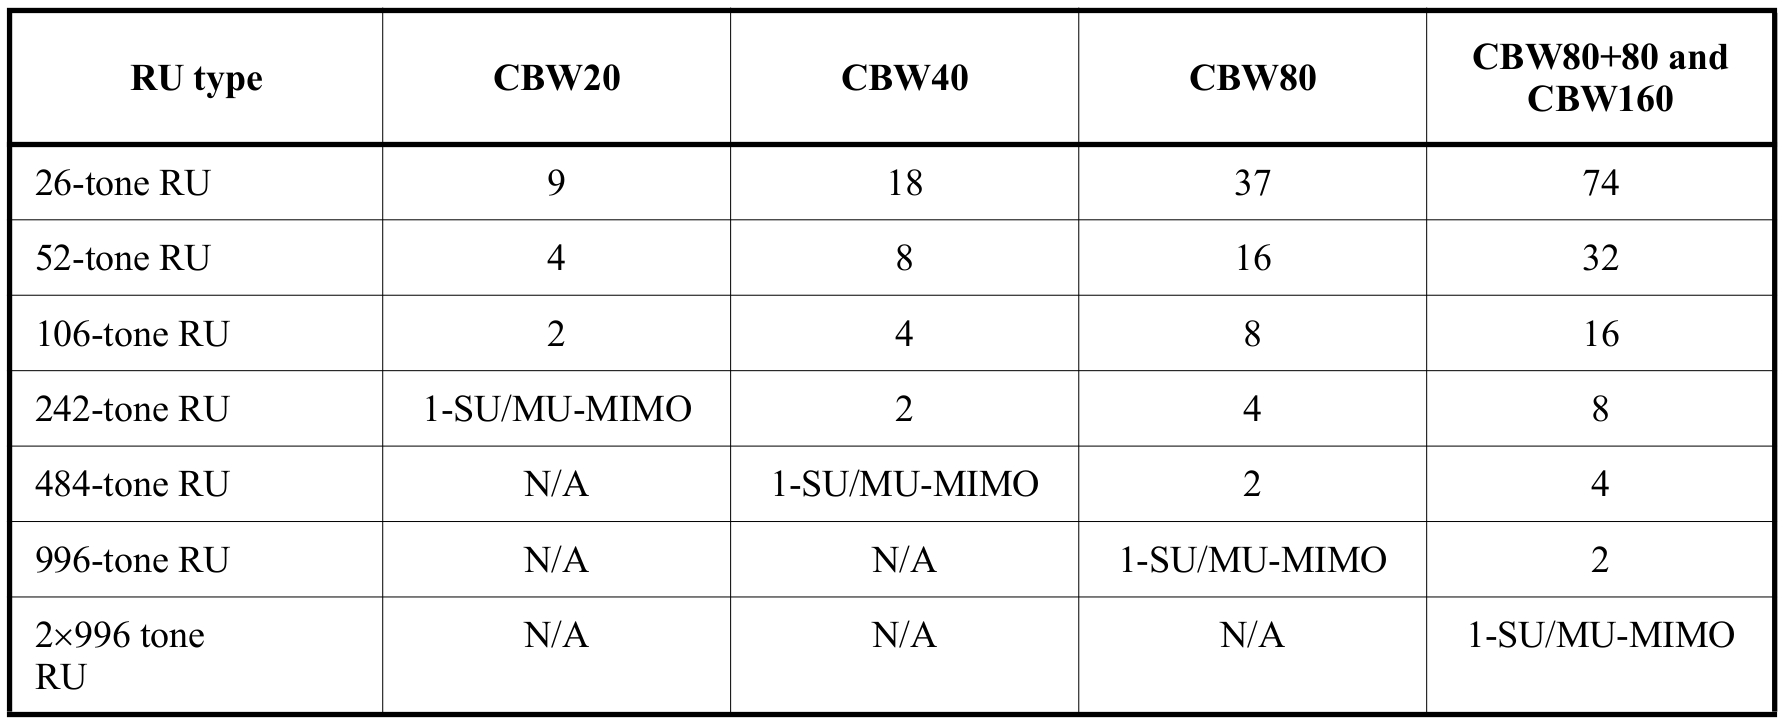
\includegraphics[scale=0.14]{./figure/RU_spec.jpg}
\caption{Maximum number of RUs for each channel width}
\label{fig_RU_spec}
\end{figure}


\begin{figure}[!t]
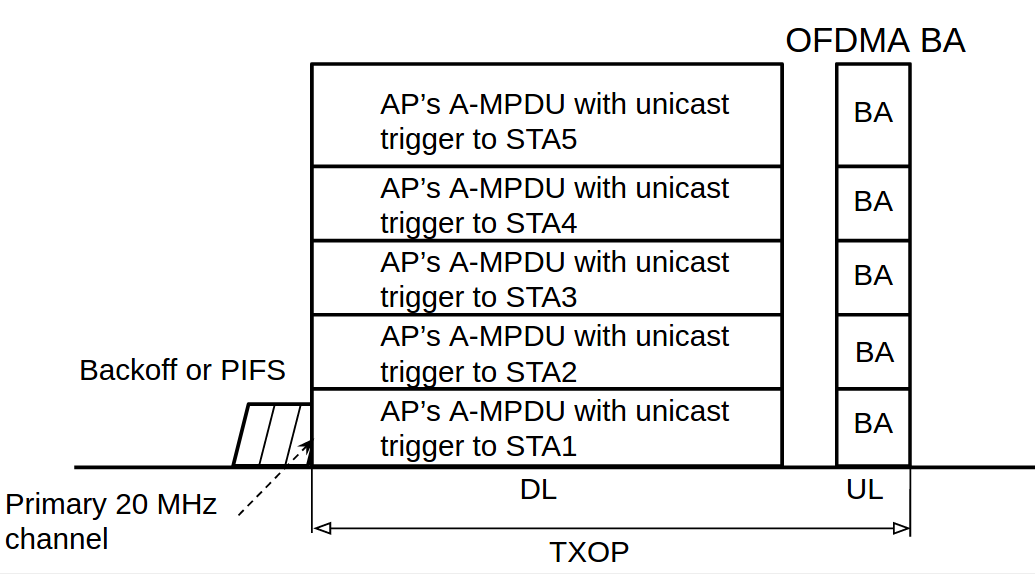
\includegraphics[scale=0.23]{./figure/fig_MU_DL.png}
\caption{MU DL of 802.11ax}
\label{fig_MU_DL}
\end{figure}


\begin{figure}[!t]
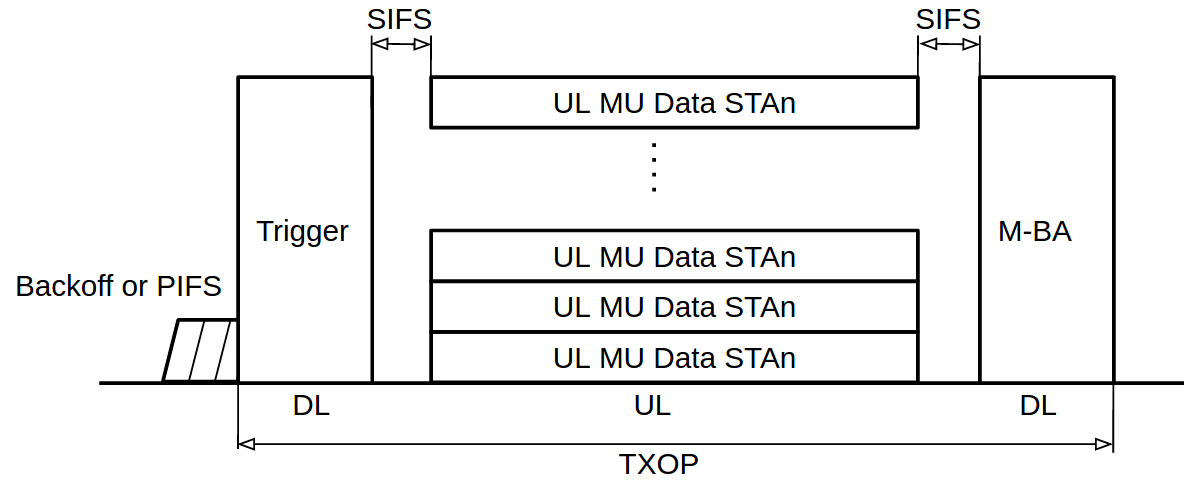
\includegraphics[scale=0.21]{./figure/fig_MU_UL.png}
\caption{Trigger-based MU UL of 802.11ax}
\label{fig_MU_UL}
\end{figure}


\subsection{MAC}
For MU DL transmission, AP will transmit DL packets to multiple stations simultaneously as in Figure \ref{fig_MU_DL}. 
The difficulty of OFDMA MU is MU UL transmission. 
Since 802.11 is not a well synchronous system, preamble and even two-way handshaking are required before a data transmission. 
A trigger-based MU UL is issued as in Figure \ref{fig_MU_UL}.
A brand new control frame, trigger frame (TF), is created to be transmitted by AP at first.
STAs could not transmit UL packets until they receive a TF which allocates RU for the STA or for random access. 
The trigger frame format is as in Figure \ref{fig_TF_format}. Since the standard is in progress, many fields remain to be determined (TBD). 
In the field \textit{User Info}, \textit{AID} represents the STA and \textit{RU Allocation} represents the RU allocated to the STA.
Especially, \textit{AID} of value 0 means the RU for random access.

\begin{figure}[!t]
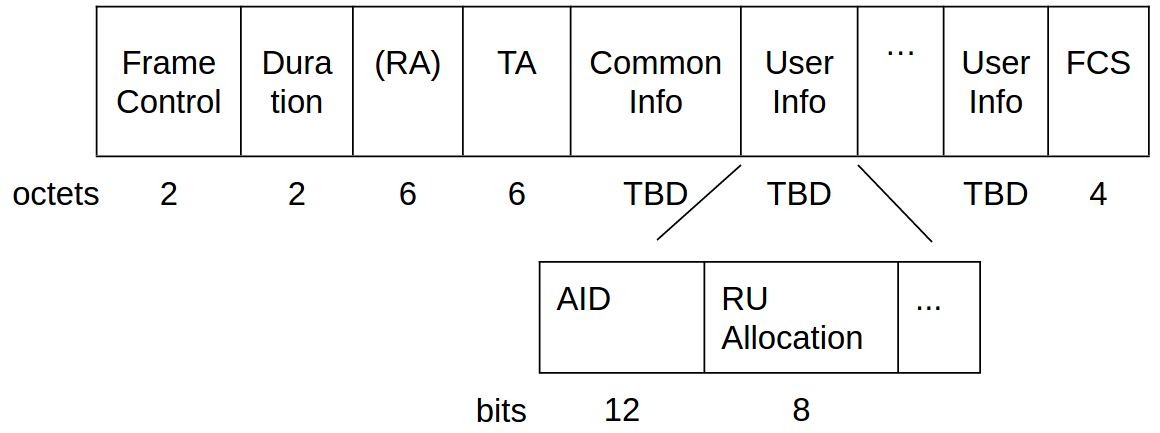
\includegraphics[scale=0.2]{./figure/fig_tf_format.png}
\caption{Trigger Frame format}
\label{fig_TF_format}
\end{figure}

%What's more, to support scheduling of TF, a mechanism called \textit{Target Wake Time} (TWT) is implemented in 802.11ax. TWT is originally issued in 802.11ah for power saving\cite{khorov2015survey}. It is also out of scope of this paper.



\subsection{OFDMA-based MCRA}		\label{sec_RA_illu}

%\begin{minipage}{.5\textwidth}
%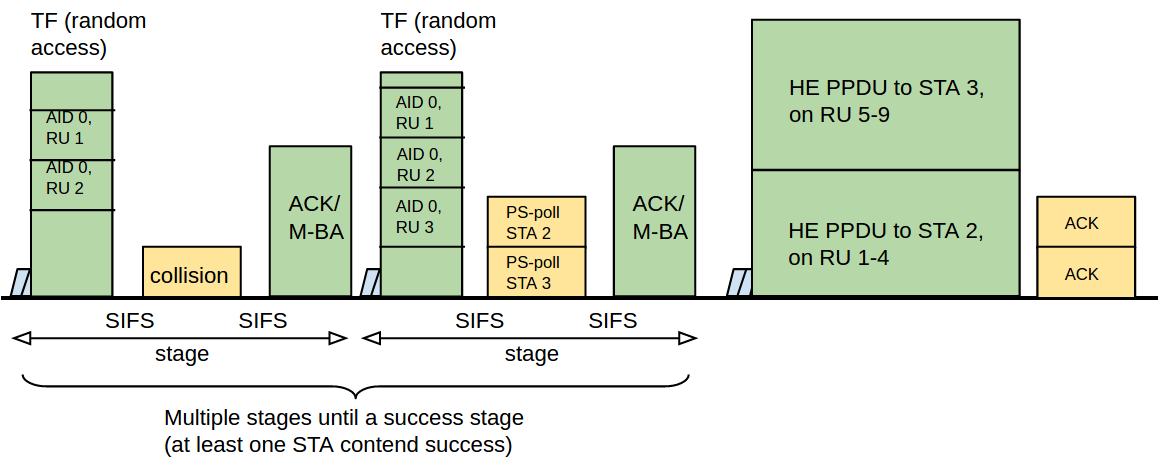
\includegraphics[scale=0.35]{./figure/RA_illu_3.png}
%\caption{Another example of OFDMA-based random access for DL in 802.11ax}
%\label{fig_ra_dl}
%\end{minipage}


\begin{figure*}[!ht]
\centering
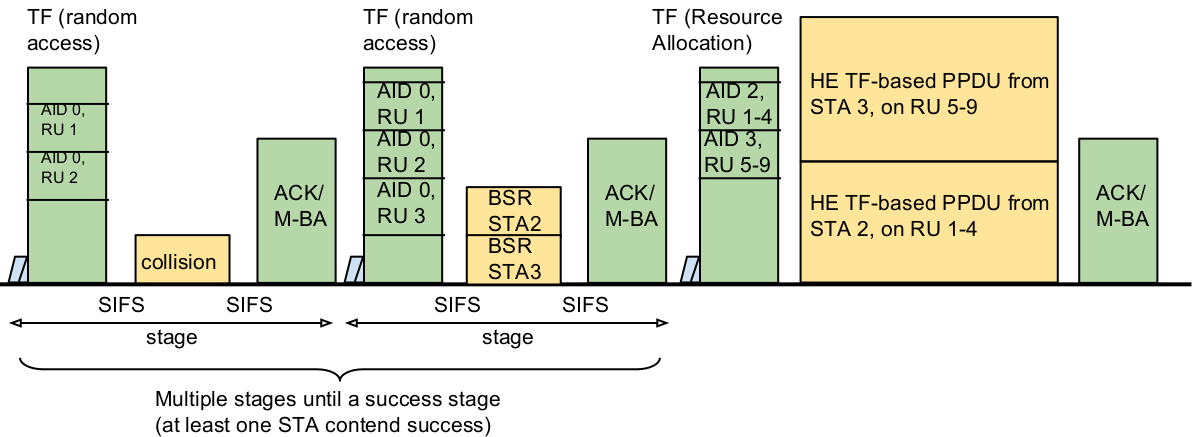
\includegraphics[scale=0.35]{./figure/RA_illu_2.png}
\caption{An example of OFDMA-based MCRA for UL in 802.11ax }
\label{fig_ra_ul}
\end{figure*}

\begin{figure*}[!ht]
%\begin{minipage}{.5\textwidth}
\centering
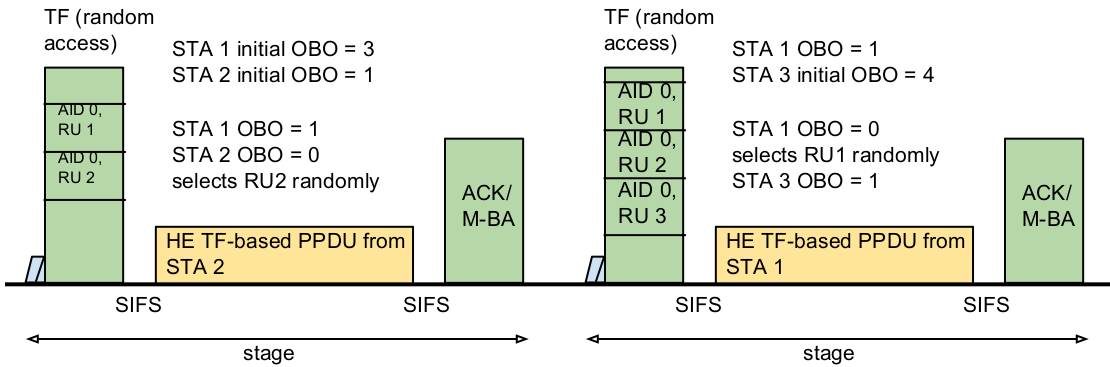
\includegraphics[scale=0.35]{./figure/RA_illu.png}
\caption{Illustration of OFDMA-based MCRA}
\label{fig_ra_illu}
%\end{minipage}
\end{figure*}
% 1. OFDMA-based MCRA is for UL
% 2. AP configure the parameters dynamically
% 3. TF-based MU UL above
% 4. detailed procedure of OFDMA-based MCRA

%Legacy IEEE 802.11 MAC is a 20 MHz SU PHY, which means that at most single user could succeed in contending at a time slot.
%With the MU PHY, HE-STA (802.11ax, high efficient station) has multiple RUs to access, which means multiple HE-STAs may access channel at the same time.
%And the parameter set is set by AP in real time.
%The procedure is of course more complicated and flexible.
%We first illustrate the ODFMA-based random access procedure then give two use cases of the random access.
We first check a use case of OFDMA-based MCRA as in Figure \ref{fig_ra_ul}.
When a STA attempts to transmit data packets, the STA will send buffer state report (BSR) frame with OFDMA-based MCRA. 
After successful contention, AP will allocate RUs for the STA by another type of trigger frame.
Then the STA transmits data packets on the allocated RUs.

Different from legacy 802.11, where all the parameters are predefined in each STA's hardware, system parameters of 802.11ax are configured dynamically by AP. 
The parameters includes $OCW_{min}, OCW_{max}, M$, where $OCW_{min}, OCW_{max}$ represent the minimum and the maximum contention window. 
And $M$ is the number of RUs for random access. 
$OCW_{min}, OCW_{max}$ are given in an element called RAPS (random access parameter set) contained in beacon frame sent by AP. 
$M$ is obtained from TF where some \textit{AID} of RUs equals 0.
OFDMA-based MCRA is thus more flexible compared with DCF.

Now let's check details by referring Figure \ref{fig_ra_illu}. 
To initialize a random access procedure, AP first transmits a TF. 
The TF announces some RUs for random access by setting the AID of those RUs value of 0. 
Attempting STAs maintain a backoff counter, called OFDMA Backoff (OBO), which are randomly generated among range $[0, OCW]$. 
Then the OBO subtracts the value of $M$ when STA receives a TF for random access. In other periods, the OBO will be frozen. 
When the OBO reaches 0, the STA will randomly select a RU from those for random access to transmit a packet after short inter-frame spacing (SIFS). 
After that, AP responds with a block ACK indicating which STAs succeed in contending. The whole three-way handshaking is called a \textit{stage}. 
A successful stage means at least one STA succeed in transmitting a request in a stage. 
It is worth reminding that the stage in this paper is a concept of time interval, not the backoff stage in other papers. 
It is specified from standard \cite{draft_ax}. 
To distinguish the two meanings, we use \textit{backoff level} in this paper replacing backoff stage.  
When STAs fail to contend, the $OCW$ will be doubled until $OCW$ reaches $OCW_{max}$. 
It means the backoff level increases until the highest level.


We look deeply into the implementation of the mechanism by checking the RAPS element as in Figure \ref{fig_RAPS}.
The two critical parameters $OCW_{min},OCW_{max}$ are specified in field \textit{OCW Range}. 
The value is defined by $OCW_{min} = 2^{EOCW_{min}}-1$, $OCW_{max} = 2^{EOCW_{max}}-1$. 
In the following analysis, we issue another parameter $m$, \textit{maximum backoff level}, so that $OCW_{max} = (OCW_{min}+1)*2^m-1$. 
Then we later specify $OCW_{max}$ with $m$ and $OCW_{min}$ in following section, which simplifies analysis.




%Another use case of random access is for power save HE-STA to solicit buffered packets at AP, which is kind of DL transmission.
%Similar to legacy 802.11 power save, HE-STA needs to transmit PS-poll or APSD-trigger frame to inform AP of its active state when the HE-STA wakes up.
%The transmission of PS-poll or APSD-trigger frame is a good case of OFDMA-based random access. After successful contention, AP will transmit the buffered packets of the HE-STA.

\begin{figure}[!h]
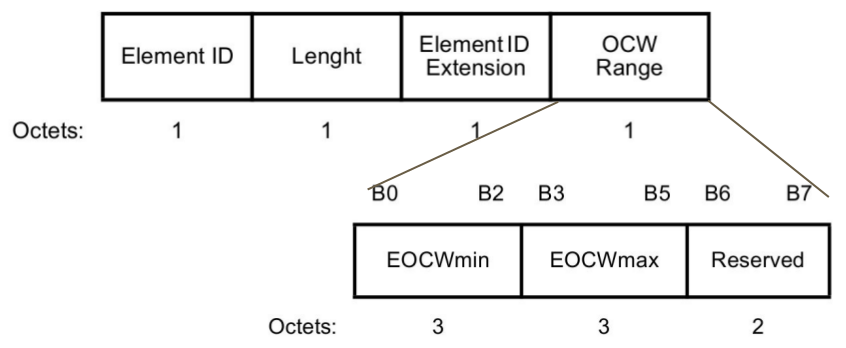
\includegraphics[scale=0.3]{./figure/RAPS.png}
\caption{Random Access Parameter Set (RAPS) Element}
\label{fig_RAPS}
\end{figure}



\section{System Model} 		\label{sec_sys_model}
Bianchi's Markov chain model could accurately depict the steady state behavior of DCF. 
It models all the details of DCF based on the assumption that at each request transmission, and regardless of the number of retransmission suffered, each request frame collides with constant and independent probability $p$. 
Although there are some great differences between OFDMA-based MCRA and DCF, the differences could be modeled by modifying the original Markov chain.
Therefore, we modify this model to conduct the saturation analysis of 802.11ax OFDMA-based MCRA also with the assumption of constant and independent conditional collision probability.

The analysis is divided into two parts. First is the Markov chain model to estimate the packet transmission probability $\tau$ and conditional collision probability $p$. 
Secondly, we evaluate the metrics given $\tau$, including number of stations who succeed in contending in a stage $n_s$, self-defined system efficiency \textit{eff}, and expected access delay of a STA $D$.  
Table \ref{table_notation} is a list of all parameters and notations.

\begin{table}[!h]
\caption{Parameters and Notations}
\centering
\label{table_notation}
\begin{tabular}{c|l}
\hline
$n$						& $\#$ of stations \\
$OCW_{min}$ ($W_0$)		& minimum OFDMA contention window \\
$OCW_{max}$ ($W_m$)		& maximum OFDMA contention window \\
$M$						& $\#$ of RUs for random access \\
$m$						& maximum backoff level \\
$p$						& packet collision probability \\
$\tau$					& station's transmission probability \\
$n_s$					& $\#$ of successful stations in a stage \\
$D$						& access delay, $\#$ of stages for a station\\
						& to contend successfully \\
\hline
\end{tabular}
\end{table}

\subsection{Packet Transmission Probability}
Consider a fixed number $n$ of stations under saturation condition, which means each station is an attempting station. 
For saturation analysis, stage of MCRA is one after another.
Thus DL transmissions does not need to be considered here.
Also, ideal channel is assumed so that collision happens only if more than one station transmit at the same RU.

DCF and OFDMA-based MCRA seem quite different from each other. 
One of the most important differences is the concept of time. In DCF, time is measured by slot. Here, we measure time by stage, the three-way handshake. 
However, they are both discrete and integer time scale. And stage does not directly reflect real time. 
The overhead of IFS and length of the request or BSR packet is not our concern. We only care about number of stages.

Similar to Bianchi's work, let $\lbrace s(t), b(t) \rbrace$ be the bi-dimension process, where $s(t)$ denotes the backoff level $(0,\cdots, m)$, and $b(t)$ denotes backoff counter $(0,W_i)$.
With the discrete and integer time scale, $t$ and $t+1$ corresponds to beginnings of two consecutive stages.
$\lbrace b(t) \rbrace$ is not Markov process, because state of the current stage does not only depend on the state of last stage. 
The bi-dimensional process $\lbrace s(t),b(t) \rbrace$ will be modeled with Markov chain.
The key assumption is still necessary that at each request transmission, and regardless of the number of retransmission suffered, each request frame collides with constant and independent probability $p$.
With the independence assumption, $p$ will be a constant. The Markov chain is able to be conducted as in Figure \ref{Markov}.

% Differences
To understand both Markov chain models of the two different mechanisms, OFDMA-based MCRA and DCF, one important concept is clarified here. 
Since stations of DCF senses the carrier before transmitting, stations may stay at a state for multiple slots. 
In OFDMA-based MCRA, a stage, a three-way handshake, contains exactly a period for a packet transmission.
Stations will subtract $M$ from the OBO only if they receive a TF for random access. 
Stations thus stay at one state for a period of exactly single stage.

% modifications
Some modifications are mentioned here to adapt to differences between OFDMA-based MCRA and DCF. 
First, in a row of states, as OBO subtracts value of $M$ rather than $1$, stations transfer to states $M$-step ahead.
Second, since states with $b(t)\leq M $ will decrease to $0$ at current state, which means stations could access RUs, we could merge these states into one state, denoted by $\lbrace i, T \rbrace$. $T$ is an integer set of $[0,M]$. 

\begin{figure*}[!t]
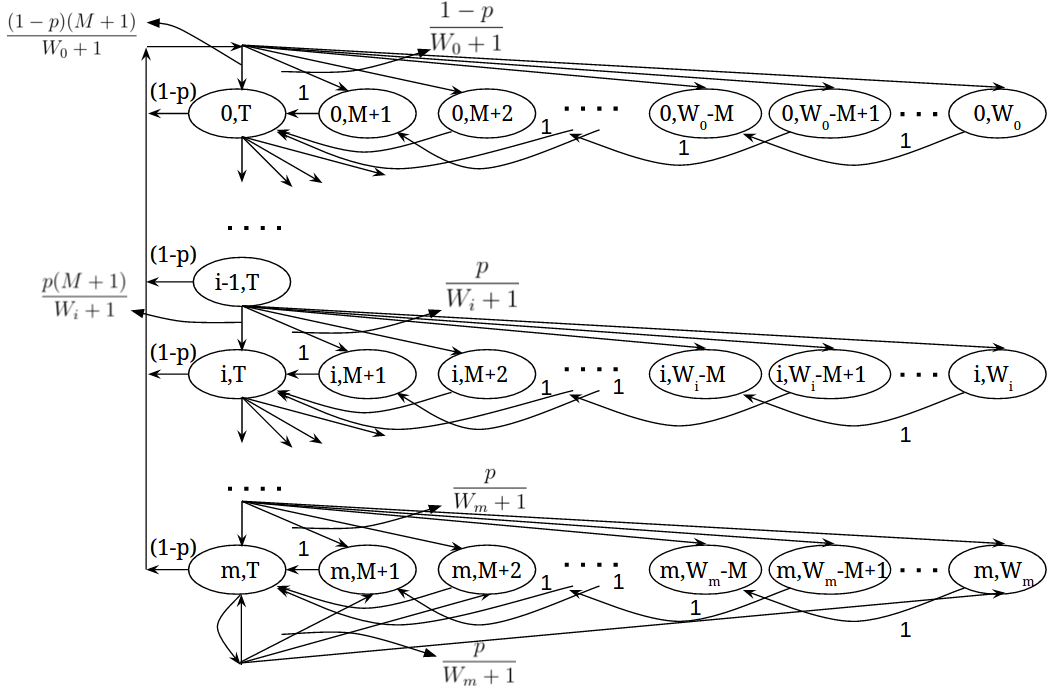
\includegraphics[scale=.45]{./figure/Markov_chain.png}
\caption{Markov Chain model for the backoff window size}
\label{Markov}
\end{figure*}

Let's assume $P\lbrace i_1, k_1|i_0,k_0\rbrace = P\lbrace s(t+1) = i_1, b(t+1)= k_1|s(t) = i_0, b(t) = k_0\rbrace $. In this Markov Chain, the only non null one-step transition probabilities are 
\begin{align}
\left\lbrace
\begin{array}{lll}
P\lbrace i, T | i, k \rbrace = 1  						& k\in [M+1,2M]			& i \in [0,m]\\ [3pt]
P\lbrace i, k-M | i, k \rbrace = 1  					& k\in [2M+1,W_i]   	& i \in [0,m]\\ [3pt]
P\lbrace 0, k | i, T \rbrace = \frac{1-p}{W_0+1}  		& k\in [M+1,W_0]		& i \in [0,m]\\ [3pt]
P\lbrace 0, T | i, T \rbrace = \frac{(1-p)(M+1)}{W_0+1} &						& i \in [0,m]\\ [3pt]
P\lbrace i, k | i-1, T \rbrace = \frac{p}{W_i+1} 		& k\in [M+1,W_i] 		& i \in [1,m]\\ [3pt]
P\lbrace i, T | i-1, T \rbrace = \frac{p(M+1)}{W_i+1}   &	  					& i \in [1,m]\\ [3pt]
P\lbrace m, k | m, T \rbrace = \frac{p}{W_m+1} 		 	& k\in [M+1,W_m] 		& \\ [3pt]
P\lbrace m, k | m, T \rbrace = \frac{p(M+1)}{W_m+1}
\end{array}
\right.
\label{trans_prob}
\end{align}

The first and second equations in (\ref{trans_prob}) accounts for the fact that the backoff counter maintained by stations will subtract $M$, the number of RUs for random access. 
The third and fourth equations represent that after a successful contention, stations will reset the contention window size to initial window size and uniformly generate a backoff value among $[0,W_0]$, since $T$ is an integer set $[0,M]$, the transition probability to states $\lbrace i, T \rbrace$ is $M+1$ times of that to states $\lbrace i, k \rbrace$. 
For the fifth and sixth equations, they represents when a failure contention occurs, the contention window size will be doubled, $W_i=2W_{i-1}+1$.
The last two equations are situation of failure contention at the maximum backoff level. 
We assume no packets are discarded, repeating retransmitting until success.

Let $b_{i,k} = \lim_{t\rightarrow \infty} P\lbrace s(t) = i, b(t) = k\rbrace,\ i\in [0,m], \ k \in [0,W_i]$, be the stationary distribution of the Markov chain. 
Then we show how to obtain transmit probability $\tau$ and conditional probability $p$.
First,  for states with $b(t) = T$, in which stations will transmit request or BSR in current stage, 
\begin{align}
b_{i-1,T}\cdot p = b_{i,T} 		\rightarrow b_{i,T} = p^i b_{0,T}, \quad 0\leq i < m \nonumber\\
b_{m-1,T}\cdot p = (1-p) b_{m,T}	\rightarrow b_{m,T} = \frac{p^m}{1-p}b_{0,T}.
\label{biT}
\end{align}

Then, other states are expressed with states of $b(t)=T$,
\begin{align}
&b_{i,k} =  \nonumber \\
&
\begin{cases}
(\lfloor \frac{W_0-k}{M} \rfloor+1)\frac{(1-p)}{W_0+1}\sum_{i=0}^m b_{i,T}, \  M+1\leq k\leq W_0,\ i = 0\\[3pt]
(\lfloor \frac{W_i-k}{M} \rfloor+1)\frac{p}{W_i+1}b_{i-1,T}, 				\	 M+1 \leq k\leq W_i, \ 0<i<m \\[3pt]
(\lfloor \frac{W_m-k}{M} \rfloor+1)\frac{p}{W_m+1} (b_{m-1,T}+b_{m,T}), 	
\end{cases}\nonumber
\\ &\qquad \qquad \qquad \qquad \quad \qquad \qquad M+1 \leq k\leq W_m, \quad i = m \nonumber \\
\label{steady_prob}
\end{align}

From (\ref{biT}), we have $\sum_{i=0}^m b_{i,T}= \frac{b_{0,T}}{1-p}$; with which, sum (\ref{steady_prob}) respectively; we obtain (\ref{part_sum}).  
\begin{figure*}[!t]

%\normalsize
%% Store the current equation number.
%\setcounter{MYtempeqncnt}{\value{equation}}
%\setcounter{equation}{4}
\begin{align}
\begin{cases}
\sum_{k=M+1}^{W_0} b_{0,k} = \frac{b_{0,T}}{W_0+1}\left(-\frac{M}{2}\left\lfloor \frac{W_0}{M}\right\rfloor ^2 + \left(W_0-\frac{M}{2}\right)\left\lfloor \frac{W_0}{M} \right\rfloor \right) \\[8pt]
\sum_{i=1}^{m-1}\sum_{k=M+1}^{W_i} b_{i,k} = \frac{b_{0,T}}{W_0+1}\left(\frac{p}{2}\right)^i \left(-\frac{M}{2}\left\lfloor \frac{W_i}{M}\right\rfloor ^2 + \left(W_i-\frac{M}{2}\right)\left\lfloor \frac{W_i}{M} \right\rfloor \right) \\[8pt]
\sum_{k=M+1}^{W_m} b_{m,k} = \frac{b_{0,T}}{W_0+1}\frac{(\frac{p}{2})^m}{1-p}\left(-\frac{M}{2}\left\lfloor \frac{W_m}{M}\right\rfloor ^2 + \left(W_m-\frac{M}{2}\right)\left\lfloor \frac{W_m}{M} \right\rfloor \right) 
\end{cases}
\label{part_sum}
\end{align}
\end{figure*}

Each subequation in (\ref{part_sum}) has the same term: $-\frac{M}{2}\left\lfloor \frac{W_i}{M}\right\rfloor ^2 + \left(W_i-\frac{M}{2}\right)\left\lfloor \frac{W_i}{M} \right\rfloor$. To simplify the expression, let $X_i = -\frac{M}{2}\left\lfloor \frac{W_i}{M}\right\rfloor ^2 + \left(W_i-\frac{M}{2}\right)\left\lfloor \frac{W_i}{M} \right\rfloor$. 
Here, we sum steady state probability of all states to get (\ref{total_sum2}).

\begin{figure*}[!t]
\begin{align}
1 &= \sum_{i=0}^m \sum_{k=0}^{W_i}b_{i,k} 
 = \frac{b_{0,T}}{W_0+1}\left( X_0 + \sum_{i=1}^{m-1}X_i\left( \frac{p}{2}\right)^i + X_m\frac{\left( \frac{p}{2}\right)^m}{1-p}\right) + \frac{b_{0,T}}{1-p}\label{total_sum}\\
& = b_{0,T}\left( \frac{(1-p)X_0+(1-p) \sum_{i=1}^{m-1}X_i\left( \frac{p}{2}\right)^i+X_m\left( \frac{p}{2}\right)^m+W_0+1}{(W_0+1)(1-p)}\right)\label{total_sum2}
\end{align}
%\setcounter{equation}{7}%{\value{MYtempeqncnt}}
%% IEEE uses as a separator
\hrulefill
\end{figure*}

Now we can express $\tau$, the probability of a station transmit a request at a randomly selected stage, as a function of $p$.

\begin{align}
\label{tau_general}
&\tau = \sum_{i=0}^m b_{i,T} = \frac{b_{0,T}}{1-p} = \nonumber \\
&\frac{W_0+1}{W_0+1+(1-p)X_0+(1-p) \sum_{i=1}^{m-1}X_i\left( \frac{p}{2}\right)^i+X_m\left( \frac{p}{2}\right)^m}
\end{align}

For $m=0, M=1$ which is SU PHY with a fixed contention window, check (\ref{total_sum}), the terms containing $X_i, i>0$ will disappear, and $b_{0,T}/(1-p)$ degrades to $b_{0,T}$.
As a result, (\ref{total_sum2}) degrades to 
\begin{align}
1 = b_{0,T}\left( \frac{W_0+1+X_0}{W_0+1}\right),
\end{align}
thereby, 
\begin{align}
\tau = b_{0,T} &= \frac{W_0+1}{W_0+1+X_0} \nonumber\\
				&= \frac{2(W_0+1)}{W_0^2+W_0+2}.
\label{tau_W0}
\end{align}
It is a little surprising at first that it is different from \cite{ho1996performance}, where $\tau=\frac{2}{W_0+1}$.
After thinking for a while, it is reasonable, because the simplified OFDMA case $M=1$ does not require carrier sensing before transmission.
It is certainly different from \cite{ho1996performance} which adopted CSMA/CA.

%Whatever, $\tau$ is independent with $n$, number of contending stations.

On the other hand, conditional collision probability $p$ has another relation with transmit probability $\tau$. 
With ideal channel assumption, collision happens only if at least one of other stations select the same RU.
Thus we have 
\begin{align}
\label{p_ax}
p = 1-\left( 1-\frac{\tau}{M} \right)^{n-1}.
\end{align}
Rewrite (\ref{p_ax}) as $\tau^\star = \left(1-(1-p)^\frac{1}{n-1} \right)M$. 
To obtain transmission probability $\tau$ and conditional collision probability $p$, we need to find solutions to group of equations \ref{tau_general} and \ref{p_ax}.
$\tau^\star(p)$ is a monotonically increasing function. 
Though $\tau(p)$ is hard to determine the monotonicity from the expression of equation \ref{tau_general} with respect to $p$. 
We justify the monotonic decrease of function \ref{tau_general} with numerical method. 
Also, $\tau(0) = \frac{W_0+1}{W_0+1+X_0}> \tau^\star(0) = 0$.
And $\tau(1) < \tau^\star(1) = M$. 
We then find the only solution with numerical method.



\subsection{Random Access Efficiency}
With the transmit probability, we could easily estimate efficiency of OFDMA-based MCRA mechanism. 
First, find expected number of stations who contend successfully to transmit request at a stage, which is denoted with $E[n_s]$. 
Extending $n_s$, we define a system efficiency as an important metric.
Secondly, we are interested in the access delay of request frame. 
In another word, say how many stages are required for a station to contend successfully, denoted by $D$.

\subsubsection{$n_s$ and System Efficiency}
What we are concerned about in the MCRA is that how many stations contend successfully during a stage, denoted by $n_s$.
Given $\tau$ and $p$, we could obtain probability that a station contend successfully in a stage, $P_{s\_station} = \tau (1-p)$.
Then, with (\ref{p_ax}), $E[n_s]$ is easily expressed as follows. 
\begin{align}
\label{equ_ns}
E[n_s] &= n P_{s\_station} \nonumber \\
		&= n\tau (1-p) \nonumber \\
		&= n\tau (1-\frac{\tau}{M})^{n-1}
\end{align}

Furthermore, normalizing $n_s$, \textit{system efficiency} here is defined as 
\begin{align}
\label{eff_def}
\textit{eff}\ (\tau) &= \frac{E[\text{number of successful stations in a given stage}]}{\text{number of RUs for random access in a stgae}} \nonumber\\
					 &=\frac{E[n_s]}{M} \nonumber \\
					 &= \frac{n\tau(1-\frac{\tau}{M})^{n-1}}{M}.
\end{align}

Both two metrics are our concerns. Another metric, access delay, is derived in next subsection.
With all these metrics, we could evaluate the performance later.

	
\subsubsection{Access Delay}
$D$, a random variable represents how many stages are required for a station to contend successfully in a stage. 
Because of saturation assumption, new request arrives once one previous request is transmitted successfully.
Thus queueing waiting time is not considered here. 
In this way, access delay $D$ follows geometric distribution with parameter $P_{s\_station}$, which is obtained just now.  
Then the expected value of access delay of request frame, $E[D]$, is 
\begin{align}
\label{equ_delay}
E[D] = \frac{1}{\tau (1-\frac{\tau}{M})^{n-1}}.
\end{align}


In a word, we focus on three metrics: number of successful stations in a stage $n_s$, system efficiency $E[n_s]/M$ and access delay given by $D$. 



\section{Model Validation} 		\label{sec_model_val}
Since we are only concerned about the OFDMA-based MCRA, to simplify the simulation, we assume STAs only solicit the OFDMA-based MCRA to transmit requests as in Figure \ref{fig_ra_illu} rather than in Figure \ref{fig_ra_ul}. 
The system parameters are set according to Figure \ref{fig_RU_spec}.
We run simulations for 100,000 stages with variety of parameter sets $\lbrace M, OCW_{min}, OCW_{max}\rbrace$ and collects the information of the two variables, number of successful attempt STAs $n_s$ and expected access delay $D$. 
The values of results from both analysis and simulation are given in figure \ref{validation} and table \ref{table_val}. 
The results show that the Markov model precisely predict the steady state behavior of the OFDMA-based MCRA mechanism.
\begin{table}[!h]
\caption{Analysis versus simulation: $n_s$ and access delay with $m=3,M=9,OCW_{min} = 15$}
\label{table_val}
\begin{center}
\begin{tabular}{c|c|c}
\hline
$n_s$ 	& analysis 	& simulation \\
\hline
$n=1$ 	& 0.72727  	& 0.72728 \\
$n=5$ 	& 2.23001	& 2.22335 \\
$n=10$	& 2.88954	& 2.88546 \\
$n=20$	& 3.29798	& 3.29857 \\
\hline
delay	& analysis	& simulation \\
\hline
$n=1$ 	& 1.37500  	& 1.37499 \\
$n=5$ 	& 2.24214	& 2.24886 \\
$n=10$	& 3.46075	& 3.46565 \\
$n=20$	& 6.06432	& 6.06323 \\
\hline
\end{tabular}
\end{center}
\end{table}

\begin{figure}[!h]
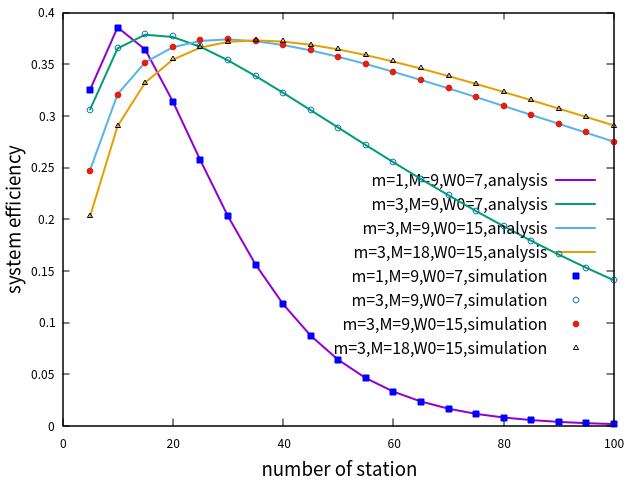
\includegraphics[scale=0.54]{./figure/multiple_parameter.png}
\caption{System efficiency: Analysis versus Simulation}
\label{validation}
\end{figure}

\section{Maximum System Efficiency and Minimum Access Delay} 	\label{sec_max_min}
With the system efficiency given in (\ref{eff_def}), we take the derivative with respect to $\tau$, and find the extreme point, $\tau^\star = M/n$. Since $\tau\in [0,1]$, $\tau^\star = min\lbrace 1,M/n\rbrace$. 
In dense scenario, i.e., the number of contending stations $n$ is large, then $\tau^\star = M/n$. 
The system efficiency thus is
\begin{align}
\textit{eff}\ (\tau^\star) = (1-\frac{1}{n})^{n-1} 
\label{equ_max_eff}
\end{align}
Then the maximum $n_s$ is 
\begin{align}
\label{equ_max_ns}
E[n_s]^\star = M \cdot \textit{eff}\ (\tau^\star) = M(1-\frac{1}{n})^{n-1} .
\end{align}
The limit of system efficiency, based on infinite $n$, is
\begin{align}
\label{eff_limit}
\lim_{n\rightarrow \infty}\textit{eff}\ (\tau^\star) = \lim_{n\rightarrow \infty}(1-\frac{1}{n})^{n-1} =\frac{1}{e} 
\end{align}

\begin{figure}[!ht]
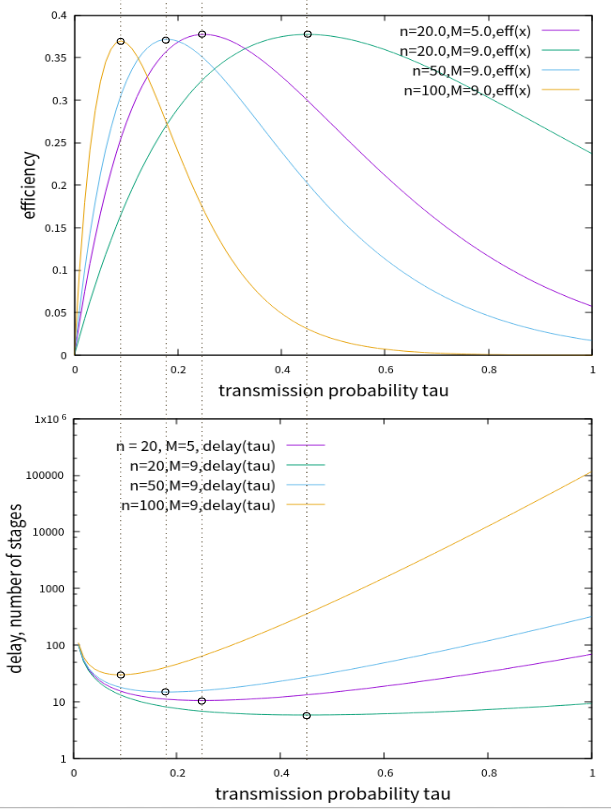
\includegraphics[scale=0.42]{./figure/chp4/max_min.png}
\caption{Efficiency and access delay versus transmission probability $\tau$}
\label{fig_eff_def}
\end{figure}


With the delay analysis given in (\ref{equ_delay}), we also take the derivative with respect to $\tau$, and find the extreme point, $\tau^\star = M/n$. Again, $\tau^\star = min\lbrace 1, M/n\rbrace$. 
When $n\geq M$, the minimum access delay is 
\begin{align}
\label{equ_min_delay}
D(\tau^\star) = \frac{n}{M(1-\frac{1}{n})^{n-1}}.
\end{align}

From above analysis, we find that the maximum system efficiency and minimum access delay are both obtained by the $\tau^\star = min\lbrace 1, M/n\rbrace$.
What's more, optimal system efficiency is independent with $M$, while $M$ affects access delay. 
The larger $M$ is, the shorter the access delay will be. 
It indicates that when AP allocates RUs for random access, the AP could allocates as many as possible, only if the channel of the RU is sensed idle by AP. 

Figure \ref{fig_eff_def} is plotted corresponding to (\ref{eff_def}) and (\ref{equ_delay}).
Consistent to the analysis above, the figure shows that the maximum system efficiency is independent of number of RUs for random access when $n\geq M$, and approaching to $1/e$ with $n$ increasing. 
What's more, the optimal transmission probability $\tau$ of system efficiency and access delay is consistent with each other, which also validates the analysis. 

Obtaining $\tau$ and $p$ by solving group equations (\ref{tau_general}) and (\ref{p_ax}), it's hard to give a closed-form of $\tau$ depending on system parameters, $M$, $W_0$, $m$ or $W_m$ and $n$.
We could only tune the system parameter set $\lbrace M, W_0, W_m \rbrace$ based on a strong assumption that $n$ is known.

\section{Performance Evaluation} 	\label{sec_perf_eval}
With above analysis, we could conveniently evaluate system efficiency and access delay by evaluating $\tau$.
Now that it is hard to directly find the relation between $\tau$ and system parameters, we could tune system parameters with a variety of system parameter sets to get some insight of the relation.


\subsection{RUs for Random Access $M$}
\label{M}
(\ref{equ_max_eff}) indicates that $M$, has nothing to do with optimal system efficiency. 
However, $n_s$ and $D$ are proportional and inversely proportional to $M$ respectively according to (\ref{equ_max_ns}) and (\ref{equ_min_delay}). 
Following analysis results validate the statement.


\begin{figure}[!t]
\centering
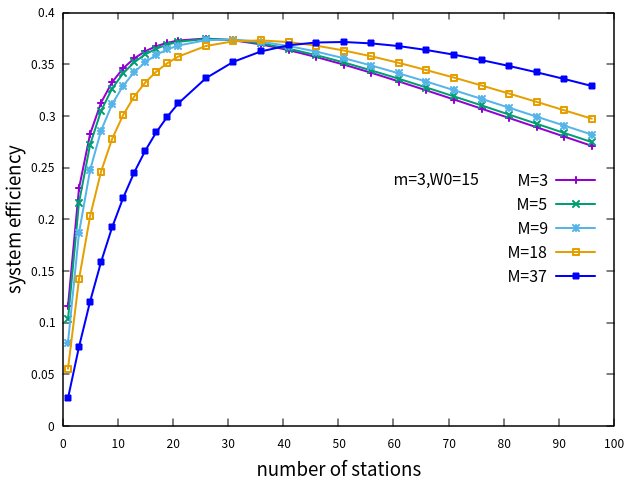
\includegraphics[scale=.54]{./figure/n_M_eff_perf.png}
\caption{System efficiency versus number of stations}
\label{fig_n_M_eff}
\end{figure}

\begin{figure}[!t]
\begin{subfigure}{0.5\textwidth}  
%\centering
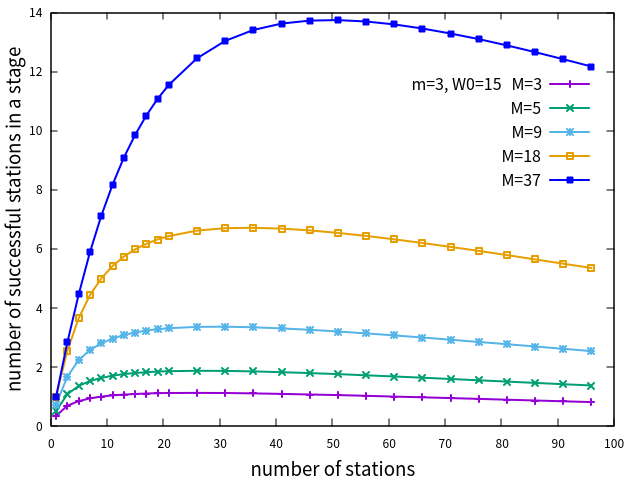
\includegraphics[scale=.54]{./figure/n_M_ns_perf.png}
\caption{Number of successful stations in a single stage versus number of stations}
\label{fig_n_M_ns}
\end{subfigure}

\begin{subfigure}{0.5\textwidth}  
%\centering
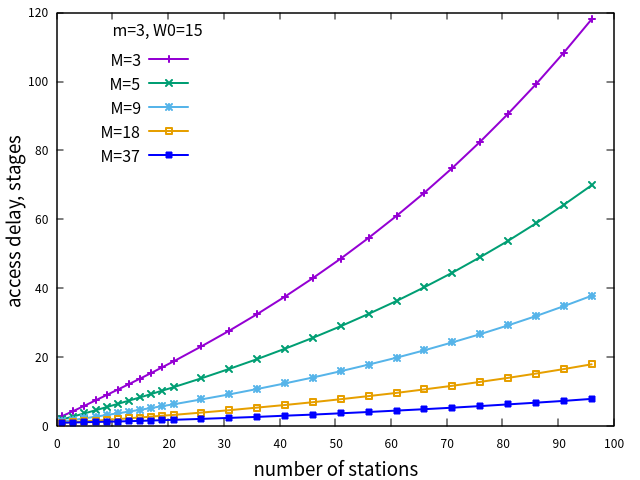
\includegraphics[scale=.54]{./figure/n_M_delay_perf.png}
\caption{Access delay versus number of stations}
\label{fig_n_M_delay}
\end{subfigure}
\caption{Configure $M$}
\end{figure}

In Figure \ref{fig_n_M_eff}, the maximum system efficiency is almost the same, approaching $1/e$. 
The only difference is "when" the optimal point will be. 
However, more practically, how many stations contend successfully in a stage?
Figure \ref{fig_n_M_ns} shows that larger $M$ results more stations contend successfully in a stage.
Moreover, Figure \ref{fig_n_M_delay} shows that larger $M$ markedly decrease the access delay. 
Above all, when AP allocates RUs for random access, AP will allocate as many RUs as possible.



\subsection{$OCW_{min}, OCW_{max}$}
\label{contend_window}

% figures
\begin{figure}[!t]
\centering
%subfigure
\begin{subfigure}{0.5\textwidth}
%\centering
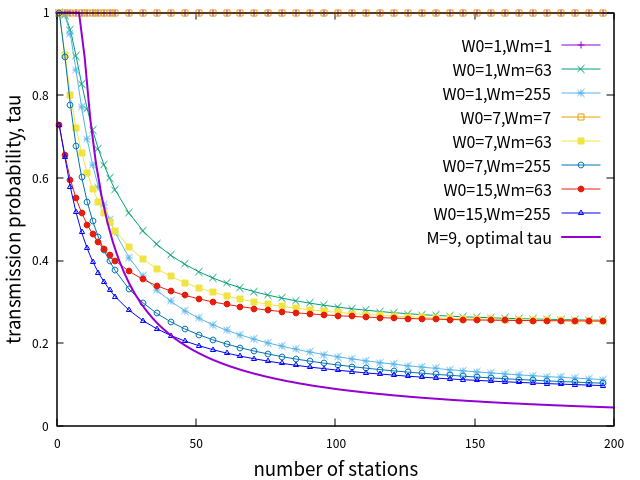
\includegraphics[scale=.54]{./figure/chp4/M9/n_tau_perf_M9_x200.png}
\caption{Case 1, given $M=9$}
\label{fig_tau_n_M9}
\end{subfigure}
%subfigure
\begin{subfigure}{0.5\textwidth}
%\centering
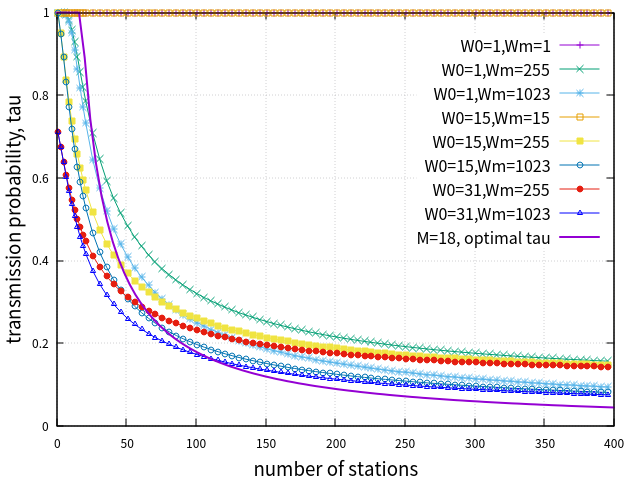
\includegraphics[scale=.54]{./figure/chp4/M18/n_tau_perf_M18_x400.png}
\caption{Case 2, given $M=18$}
\label{fig_tau_n_M18}
\end{subfigure}
%caption
\caption{Transmission probability versus number of stations}
\label{fig_tau_n}
\end{figure}
% should have sth beginning
%For those $m>0$, the curve will be convex and monotone decreasing. It is intuitive that with the increasing number of stations, the transmit probability decreases.
Figure \ref{fig_tau_n} shows case 1 ($M=9$) and case 2 ($M=18$), so that the rules we get are more convinced.
In the figure, the purple line without point depicts the optimal $\tau$, which is given according to $\tau^\star = min\lbrace 1, M/n \rbrace$.
With above analysis and effects of $M$, we tune remaining parameters $OCW_{min}, OCW_{max}$ so that $\tau$ approaches the optimal line. 
To see the trend of line, we give larger $n$. Then some rules could obtained as follows.

First, the $OCW_{min}$ or $W_0$, determines $\tau$ of loose scenario. 
The larger $W_0$ is, the lower $\tau$ is at $n=1$.
That's why cases in Figure \ref{fig_tau_n} have two different start points.

Secondly, $m=0$ results in constant $\tau$, which is consistent with (\ref{tau_W0}) that $\tau$ does not depend on $n$.
A special case is $W_0<M$ for scenario $n\leq M$, it results in constant transmission probability equals to 1 regardless of $n$. 
It perfectly matches $\tau^\star$ at $n\leq M$ as $\tau^\star = 1$ for the scenario $n \leq M$.
Thus, if given $n\leq M$, the optimal configuration will be $OCW_{max}= OCW_{min} < M$. 


Thirdly, $W_m$ affects more on dense scenario.
It determines the limit of the $\tau$, i.e., where the line of $\tau$ will converge. 
Lines with the same $W_m$ will converge to a same value. 
And both the two figures in Figure \ref{fig_tau_n} correspond with the above statement.
And larger $W_m$ causes lower $\tau$, which is closer to $\tau^\star$ when $n$ is large. 
 


% figures
\begin{figure}[!t]
\centering
\begin{subfigure}{0.5\textwidth}
\centering
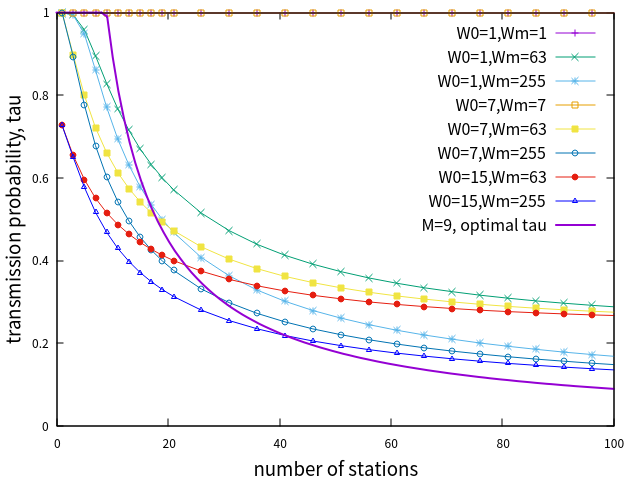
\includegraphics[scale=.54]{./figure/chp4/M9/n_tau_perf_M9_x100.png}
\caption{Case 1, given $M=9$}
\label{fig_tau_n_M9_detail}
\end{subfigure}

\begin{subfigure}{0.5\textwidth}
\centering
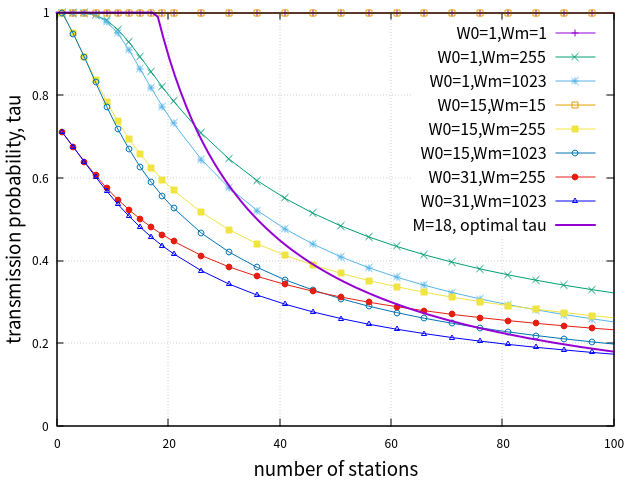
\includegraphics[scale=.54]{./figure/chp4/M18/n_tau_perf_M18_x100.png}
\caption{Case 2, given $M=18$}
\label{fig_tau_n_M18_detail}
\end{subfigure}

\caption{Details of transmission probability versus number of stations when $n\leq 100$}
\label{fig_tau_n_detail}
\end{figure}

Then, we draw two subfigures with x axis range $[0,100]$ to observe more clearly as in Figure \ref{fig_tau_n_detail}. 
From the two subfigures \ref{fig_tau_n_M9_detail} and \ref{fig_tau_n_M18_detail} we find another rule that when $W_0=1$, line of $\tau$ will have a flat start.
It happens that the flat start matches better with $\tau^\star$ when $n\leq M$.

Based on all above observations, we conclude that $W_0$ has significant influence on scenario of $n\leq M$, while $W_m$ counts when $n$ is large or $n>M$. 
In the next two subsections, we practically check the system efficiency and access delay under different parameter configurations of $\lbrace W_0, W_m \rbrace$, with which we could find explicit relation between the parameter and performance.




\subsubsection{Configure $OCW_{max}$}

\begin{figure}[!t]
\centering
\begin{subfigure}{0.5\textwidth}  
  \centering  
  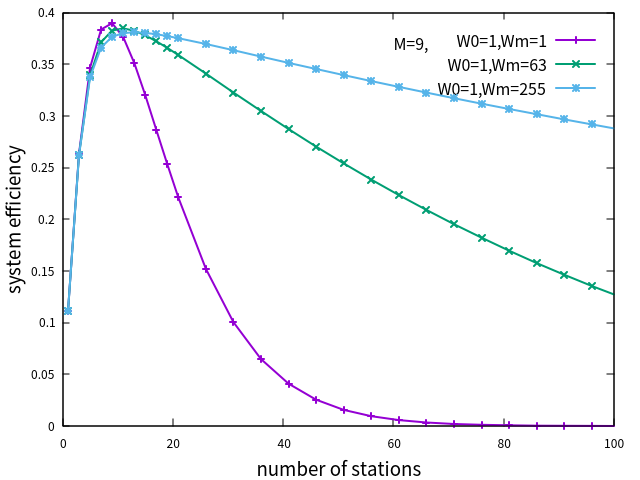
\includegraphics[scale=0.54]{./figure/chp4/M9/n_eff_perf_W01.png}  
    \caption{System efficiency versus number of stations}   
    \label{fig_n_eff_Wm}
\end{subfigure}   

\begin{subfigure}{0.5\textwidth}
	\centering
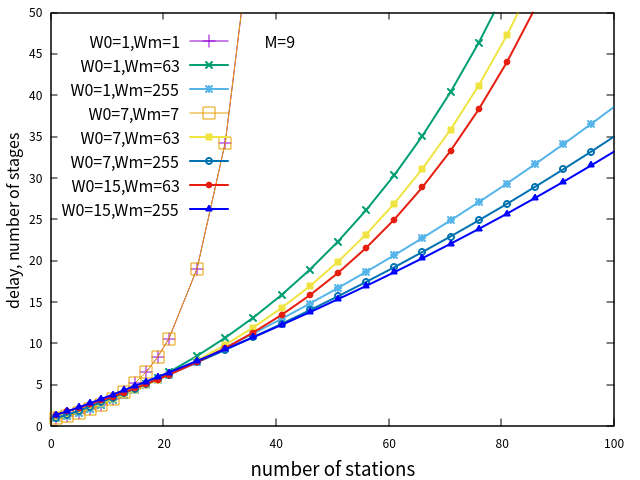
\includegraphics[scale=.54]{./figure/chp4/M9/n_delay_perf.png}
\caption{Access delay versus number of stations}
\label{fig_n_delay_Wm}
\end{subfigure}
\caption{Example of Configuring $OCW_{max}$, given $M=9$}
\end{figure}

With above rough rules, we estimate the effects of $OCW_{max}$ first by setting different $OCW_{max}$ while given $OCW_{min}=1$ and $M=9$.
Actually the data we use to generate the figures are the same with that for Figure \ref{fig_tau_n_M9}. 
In Figure \ref{fig_n_eff_Wm}, we select three of them to clearly display the effect of $OCW_{max}$ on system efficiency.
From the figure, it is obvious that larger $OCW_{max}$ is much better for system efficiency when $n\geq M$. 
The result corresponds to the above rules we obtain from effect of parameters on $\tau$.
Additionally, $OCW_{max}$ has the same effect on access delay . And since we use the same data with that in figure \ref{fig_tau_n_M9}, we find that the lines which converge in figure \ref{fig_tau_n_M9} also have the same tendency in figure \ref{fig_n_delay_Wm}. 

As stated in previous section that $OCW_{max}$ has significant influence on scenario of $n\geq M$. 
With increasing $n$, larger $OCW_{max}$ will obtain larger gain. 


\subsubsection{Configure $OCW_{min}$}

\begin{figure}[!t]
\centering
\begin{subfigure}{0.5\textwidth}  
  \centering  
  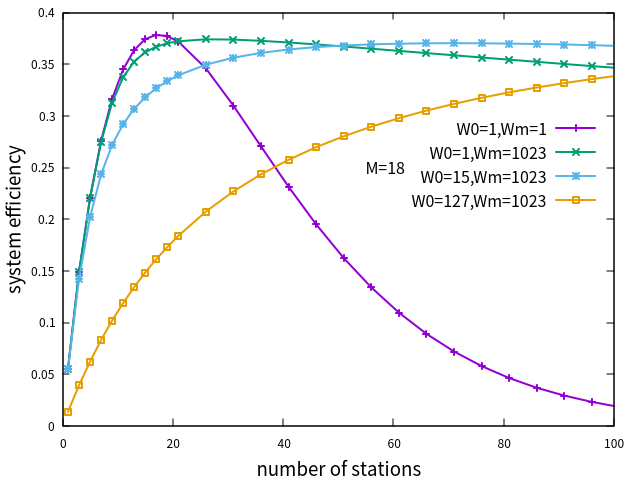
\includegraphics[scale=0.54]{./figure/chp4/M18/n_eff_perf_Wm1023.png}  
    \caption{System efficiency versus number of stations}   
    \label{fig_n_eff_W0}
\end{subfigure}   

\begin{subfigure}{0.5\textwidth}
	\centering
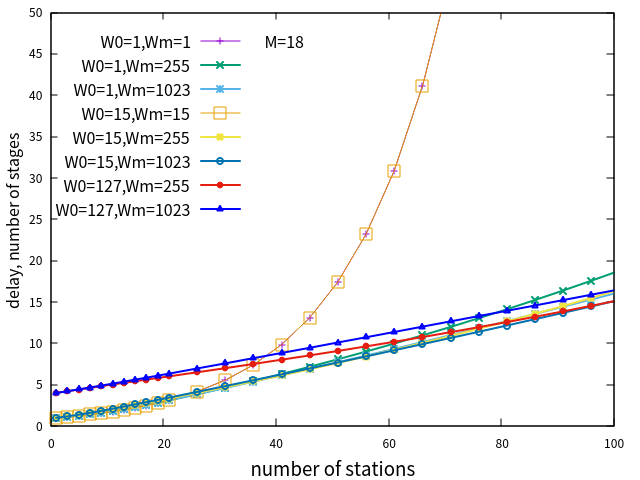
\includegraphics[scale=.54]{./figure/chp4/M18/n_delay_perf.png}
\caption{Access delay versus number of stations}
\label{fig_n_delay_W0}
\end{subfigure}
\caption{Example of Configuring $OCW_{min}$, given $M=18$}
\end{figure}

To estimate the effect of $OCW_{min}$, we compare the performance of different configurations of $OCW_{min}$ while given $OCW_{max}=1023$, which has been validated that larger $OCW_{max}$ is better, and $M=18$. 
First, as we claim in Section \ref{contend_window} that $W_0=W_m\leq M$ is the perfect configuration in scenario of $n\leq M$, it is validated here that maximum system efficiency and minimum access delay are achieved with the configuration in scenario of $n\leq M$.
However, configuration of small $OCW_{min}$ and large $OCW_{max}$ almost achieves as good performance as the perfect configuration.  
Secondly, $OCW_{min}$ determines the start of line, and it has significant influence on scenario of $n\leq M$.
From Figure \ref{fig_n_eff_W0} and \ref{fig_n_delay_W0}, we find larger $OCW_{min}=127$ has lower system efficiency and larger access delay. 

Now, we summarize above rules as follows.
 
\begin{itemize}
\item[1] For $M$: the larger the better
\item[2] For $OCW_{min}, OCW_{max}$:
	\begin{itemize}
	\item $OCW_{min}$ counts when $n\leq M$. Smaller $OCW_{min}$ is better.
	\item $OCW_{max}$ counts when $n>M$. Larger $OCW_{max}$ is better.
	\end{itemize}
\end{itemize}
\begin{itemize}
	\item Special case: for $n\leq M$\\
	$OCW_{max}=OCW_{min}<M$ 
\end{itemize}





\section{Conclusion}   \label{sec_conclu}
In this paper, we evaluate performance of the new OFDMA-based MCRA mechanism of 802.11ax.
We extends \cite{bianchi2000performance} to model the MCRA mechanism and conduct a saturation analysis.
The simple Markov model is validated that it could also precisely depict the steady state behavior of OFDMA-based MCRA of 802.11ax.
With the model, we derive the expression of system efficiency and access delay. 
Performance strongly depends on various system parameters.
The number of RUs or subchannels is as large as possible.
The initial contention window counts when only few stations exist, while maximum contention window is important in dense scenario.

Different from DCF of legacy 802.11, the OFDMA-based MCRA mechanism is more flexible, with system parameters dynamically configured.
An real-time algorithm is required to configure the system parameters dynamically. 
This paper takes the first step to catch some insight from the steady state behavior of the MCRA mechanism.
In the future, transient analysis is necessary to generate a configuration algorithm.

%An interesting result is that the maximum system efficiency and minimum access delay are obtained by the same transmission probability $\tau$, which is given by $\tau^\star = min \lbrace 1,M/n\rbrace$. 
%Then rules of configuration of parameter set aimed at reaching the optimal transmission probability $\tau^\star$ is proposed for AP according to system state, mainly the number of contending stations. 
%The last group cases of various parameter sets validates our proposed rules.

%We find an interesting result that system efficiency and access delay behave consistent with each other and they both strongly depend on the system parameters.
%Larger $M$ is better whenever $n$ is large or small.
%Smaller $OCW_{min}$ is better and affects more in case when $n$ is small.
%Larger $OCW_{max}$ is better and affcets more in case when $n$ is large. 
%Especially, an optimal configuration $OCW_{min}=OCW_{max}\leq M$ fits in case $n\leq M$. 
%All above are the rough insight we obtain from steady state behavior.
%To generate a dynamic algorithm to configure the system parameters requires transient analysis, which could be done in the future.

% An example of a floating figure using the graphicx package.
% Note that \label must occur AFTER (or within) \caption.
% For figures, \caption should occur after the \includegraphics.
% Note that IEEEtran v1.7 and later has special internal code that
% is designed to preserve the operation of \label within \caption
% even when the captionsoff option is in effect. However, because
% of issues like this, it may be the safest practice to put all your
% \label just after \caption rather than within \caption{}.
%
% Reminder: the "draftcls" or "draftclsnofoot", not "draft", class
% option should be used if it is desired that the figures are to be
% displayed while in draft mode.
%
%\begin{figure}[!t]
%\centering
%\includegraphics[width=2.5in]{myfigure}
% where an .eps filename suffix will be assumed under latex, 
% and a .pdf suffix will be assumed for pdflatex; or what has been declared
% via \DeclareGraphicsExtensions.
%\caption{Simulation results for the network.}
%\label{fig_sim}
%\end{figure}

% Note that the IEEE typically puts floats only at the top, even when this
% results in a large percentage of a column being occupied by floats.


% An example of a double column floating figure using two subfigures.
% (The subfig.sty package must be loaded for this to work.)
% The subfigure \label commands are set within each subfloat command,
% and the \label for the overall figure must come after \caption.
% \hfil is used as a separator to get equal spacing.
% Watch out that the combined width of all the subfigures on a 
% line do not exceed the text width or a line break will occur.
%
%\begin{figure*}[!t]
%\centering
%\subfloat[Case I]{\includegraphics[width=2.5in]{box}%
%\label{fig_first_case}}
%\hfil
%\subfloat[Case II]{\includegraphics[width=2.5in]{box}%
%\label{fig_second_case}}
%\caption{Simulation results for the network.}
%\label{fig_sim}
%\end{figure*}
%
% Note that often IEEE papers with subfigures do not employ subfigure
% captions (using the optional argument to \subfloat[]), but instead will
% reference/describe all of them (a), (b), etc., within the main caption.
% Be aware that for subfig.sty to generate the (a), (b), etc., subfigure
% labels, the optional argument to \subfloat must be present. If a
% subcaption is not desired, just leave its contents blank,
% e.g., \subfloat[].


% An example of a floating table. Note that, for IEEE style tables, the
% \caption command should come BEFORE the table and, given that table
% captions serve much like titles, are usually capitalized except for words
% such as a, an, and, as, at, but, by, for, in, nor, of, on, or, the, to
% and up, which are usually not capitalized unless they are the first or
% last word of the caption. Table text will default to \footnotesize as
% the IEEE normally uses this smaller font for tables.
% The \label must come after \caption as always.
%
%\begin{table}[!t]
%% increase table row spacing, adjust to taste
%\renewcommand{\arraystretch}{1.3}
% if using array.sty, it might be a good idea to tweak the value of
% \extrarowheight as needed to properly center the text within the cells
%\caption{An Example of a Table}
%\label{table_example}
%\centering
%% Some packages, such as MDW tools, offer better commands for making tables
%% than the plain LaTeX2e tabular which is used here.
%\begin{tabular}{|c||c|}
%\hline
%One & Two\\
%\hline
%Three & Four\\
%\hline
%\end{tabular}
%\end{table}


% Note that the IEEE does not put floats in the very first column
% - or typically anywhere on the first page for that matter. Also,
% in-text middle ("here") positioning is typically not used, but it
% is allowed and encouraged for Computer Society conferences (but
% not Computer Society journals). Most IEEE journals/conferences use
% top floats exclusively. 
% Note that, LaTeX2e, unlike IEEE journals/conferences, places
% footnotes above bottom floats. This can be corrected via the
% \fnbelowfloat command of the stfloats package.





% if have a single appendix:
%\appendix[Proof of the Zonklar Equations]
% or
%\appendix  % for no appendix heading
% do not use \section anymore after \appendix, only \section*
% is possibly needed

% use appendices with more than one appendix
% then use \section to start each appendix
% you must declare a \section before using any
% \subsection or using \label (\appendices by itself
% starts a section numbered zero.)
%


\appendices
%\section{Proof of the First Zonklar Equation}
%Appendix one text goes here.

% you can choose not to have a title for an appendix
% if you want by leaving the argument blank
%\section{}
%Appendix two text goes here.


% use section* for acknowledgment
%\section*{Acknowledgment}


%The authors would like to thank...


% Can use something like this to put references on a page
% by themselves when using endfloat and the captionsoff option.
\ifCLASSOPTIONcaptionsoff
  \newpage
\fi



% trigger a \newpage just before the given reference
% number - used to balance the columns on the last page
% adjust value as needed - may need to be readjusted if
% the document is modified later
%\IEEEtriggeratref{8}
% The "triggered" command can be changed if desired:
%\IEEEtriggercmd{\enlargethispage{-5in}}

% references section

% can use a bibliography generated by BibTeX as a .bbl file
% BibTeX documentation can be easily obtained at:
% http://mirror.ctan.org/biblio/bibtex/contrib/doc/
% The IEEEtran BibTeX style support page is at:
% http://www.michaelshell.org/tex/ieeetran/bibtex/
\bibliographystyle{IEEEtran}
% argument is your BibTeX string definitions and bibliography database(s)
\bibliography{formula.bib}
%
% <OR> manually copy in the resultant .bbl file
% set second argument of \begin to the number of references
% (used to reserve space for the reference number labels box)
%\begin{thebibliography}{1}

%\bibitem{IEEEhowto:kopka}
%H.~Kopka and P.~W. Daly, \emph{A Guide to \LaTeX}, 3rd~ed.\hskip 1em plus
%  0.5em minus 0.4em\relax Harlow, England: Addison-Wesley, 1999.

%\end{thebibliography}

% biography section
% 
% If you have an EPS/PDF photo (graphicx package needed) extra braces are
% needed around the contents of the optional argument to biography to prevent
% the LaTeX parser from getting confused when it sees the complicated
% \includegraphics command within an optional argument. (You could create
% your own custom macro containing the \includegraphics command to make things
% simpler here.)
%\begin{IEEEbiography}[{\includegraphics[width=1in,height=1.25in,clip,keepaspectratio]{mshell}}]{Michael Shell}
% or if you just want to reserve a space for a photo:

\begin{IEEEbiography}{Michael Shell}
Biography text here.
\end{IEEEbiography}

% if you will not have a photo at all:
\begin{IEEEbiographynophoto}{John Doe}
Biography text here.
\end{IEEEbiographynophoto}

% insert where needed to balance the two columns on the last page with
% biographies
%\newpage

\begin{IEEEbiographynophoto}{Jane Doe}
Biography text here.
\end{IEEEbiographynophoto}

% You can push biographies down or up by placing
% a \vfill before or after them. The appropriate
% use of \vfill depends on what kind of text is
% on the last page and whether or not the columns
% are being equalized.

%\vfill

% Can be used to pull up biographies so that the bottom of the last one
% is flush with the other column.
%\enlargethispage{-5in}



% that's all folks
\end{document}


